\documentclass[twoside]{book}

% Packages required by doxygen
\usepackage{fixltx2e}
\usepackage{calc}
\usepackage{doxygen}
\usepackage[export]{adjustbox} % also loads graphicx
\usepackage{graphicx}
\usepackage[utf8]{inputenc}
\usepackage{makeidx}
\usepackage{multicol}
\usepackage{multirow}
\PassOptionsToPackage{warn}{textcomp}
\usepackage{textcomp}
\usepackage[nointegrals]{wasysym}
\usepackage[table]{xcolor}

% Font selection
\usepackage[T1]{fontenc}
\usepackage[scaled=.90]{helvet}
\usepackage{courier}
\usepackage{amssymb}
\usepackage{sectsty}
\renewcommand{\familydefault}{\sfdefault}
\allsectionsfont{%
  \fontseries{bc}\selectfont%
  \color{darkgray}%
}
\renewcommand{\DoxyLabelFont}{%
  \fontseries{bc}\selectfont%
  \color{darkgray}%
}
\newcommand{\+}{\discretionary{\mbox{\scriptsize$\hookleftarrow$}}{}{}}

% Page & text layout
\usepackage{geometry}
\geometry{%
  a4paper,%
  top=2.5cm,%
  bottom=2.5cm,%
  left=2.5cm,%
  right=2.5cm%
}
\tolerance=750
\hfuzz=15pt
\hbadness=750
\setlength{\emergencystretch}{15pt}
\setlength{\parindent}{0cm}
\setlength{\parskip}{3ex plus 2ex minus 2ex}
\makeatletter
\renewcommand{\paragraph}{%
  \@startsection{paragraph}{4}{0ex}{-1.0ex}{1.0ex}{%
    \normalfont\normalsize\bfseries\SS@parafont%
  }%
}
\renewcommand{\subparagraph}{%
  \@startsection{subparagraph}{5}{0ex}{-1.0ex}{1.0ex}{%
    \normalfont\normalsize\bfseries\SS@subparafont%
  }%
}
\makeatother

% Headers & footers
\usepackage{fancyhdr}
\pagestyle{fancyplain}
\fancyhead[LE]{\fancyplain{}{\bfseries\thepage}}
\fancyhead[CE]{\fancyplain{}{}}
\fancyhead[RE]{\fancyplain{}{\bfseries\leftmark}}
\fancyhead[LO]{\fancyplain{}{\bfseries\rightmark}}
\fancyhead[CO]{\fancyplain{}{}}
\fancyhead[RO]{\fancyplain{}{\bfseries\thepage}}
\fancyfoot[LE]{\fancyplain{}{}}
\fancyfoot[CE]{\fancyplain{}{}}
\fancyfoot[RE]{\fancyplain{}{\bfseries\scriptsize Generated by Doxygen }}
\fancyfoot[LO]{\fancyplain{}{\bfseries\scriptsize Generated by Doxygen }}
\fancyfoot[CO]{\fancyplain{}{}}
\fancyfoot[RO]{\fancyplain{}{}}
\renewcommand{\footrulewidth}{0.4pt}
\renewcommand{\chaptermark}[1]{%
  \markboth{#1}{}%
}
\renewcommand{\sectionmark}[1]{%
  \markright{\thesection\ #1}%
}

% Indices & bibliography
\usepackage{natbib}
\usepackage[titles]{tocloft}
\setcounter{tocdepth}{3}
\setcounter{secnumdepth}{5}
\makeindex

% Hyperlinks (required, but should be loaded last)
\usepackage{ifpdf}
\ifpdf
  \usepackage[pdftex,pagebackref=true]{hyperref}
\else
  \usepackage[ps2pdf,pagebackref=true]{hyperref}
\fi
\hypersetup{%
  colorlinks=true,%
  linkcolor=blue,%
  citecolor=blue,%
  unicode%
}

% Custom commands
\newcommand{\clearemptydoublepage}{%
  \newpage{\pagestyle{empty}\cleardoublepage}%
}

\usepackage{caption}
\captionsetup{labelsep=space,justification=centering,font={bf},singlelinecheck=off,skip=4pt,position=top}

%===== C O N T E N T S =====

\begin{document}

% Titlepage & ToC
\hypersetup{pageanchor=false,
             bookmarksnumbered=true,
             pdfencoding=unicode
            }
\pagenumbering{roman}
\begin{titlepage}
\vspace*{7cm}
\begin{center}%
{\Large Plume Creator Data \\[1ex]\large 1.\+60 }\\
\vspace*{1cm}
{\large Generated by Doxygen 1.8.11}\\
\end{center}
\end{titlepage}
\clearemptydoublepage
\tableofcontents
\clearemptydoublepage
\pagenumbering{arabic}
\hypersetup{pageanchor=true}

%--- Begin generated contents ---
\chapter{Hierarchical Index}
\section{Class Hierarchy}
This inheritance list is sorted roughly, but not completely, alphabetically\+:\begin{DoxyCompactList}
\item \contentsline{section}{P\+L\+M\+Db\+Error}{\pageref{struct_p_l_m_db_error}}{}
\item \contentsline{section}{P\+L\+M\+Db\+Paper}{\pageref{class_p_l_m_db_paper}}{}
\item \contentsline{section}{P\+L\+M\+Db\+Tree}{\pageref{class_p_l_m_db_tree}}{}
\item \contentsline{section}{P\+L\+M\+Error}{\pageref{struct_p_l_m_error}}{}
\item Q\+Object\begin{DoxyCompactList}
\item \contentsline{section}{P\+L\+M\+Data}{\pageref{class_p_l_m_data}}{}
\item \contentsline{section}{P\+L\+M\+Error\+Hub}{\pageref{class_p_l_m_error_hub}}{}
\item \contentsline{section}{P\+L\+M\+Exporter}{\pageref{class_p_l_m_exporter}}{}
\item \contentsline{section}{P\+L\+M\+Importer}{\pageref{class_p_l_m_importer}}{}
\item \contentsline{section}{P\+L\+M\+Project}{\pageref{class_p_l_m_project}}{}
\item \contentsline{section}{P\+L\+M\+Project\+Hub}{\pageref{class_p_l_m_project_hub}}{}
\item \contentsline{section}{P\+L\+M\+Project\+Manager}{\pageref{class_p_l_m_project_manager}}{}
\item \contentsline{section}{P\+L\+M\+Property}{\pageref{class_p_l_m_property}}{}
\item \contentsline{section}{P\+L\+M\+Signal\+Hub}{\pageref{class_p_l_m_signal_hub}}{}
\item \contentsline{section}{P\+L\+M\+Task}{\pageref{class_p_l_m_task}}{}
\begin{DoxyCompactList}
\item \contentsline{section}{P\+L\+M\+Project\+Close\+All\+Projects}{\pageref{class_p_l_m_project_close_all_projects}}{}
\item \contentsline{section}{P\+L\+M\+Project\+Close\+Project}{\pageref{class_p_l_m_project_close_project}}{}
\item \contentsline{section}{P\+L\+M\+Project\+Get\+Project\+Id\+List}{\pageref{class_p_l_m_project_get_project_id_list}}{}
\item \contentsline{section}{P\+L\+M\+Project\+Load\+Project}{\pageref{class_p_l_m_project_load_project}}{}
\item \contentsline{section}{P\+L\+M\+Write\+Get\+All}{\pageref{class_p_l_m_write_get_all}}{}
\item \contentsline{section}{P\+L\+M\+Write\+Get\+All\+Indents}{\pageref{class_p_l_m_write_get_all_indents}}{}
\item \contentsline{section}{P\+L\+M\+Write\+Get\+All\+Titles}{\pageref{class_p_l_m_write_get_all_titles}}{}
\item \contentsline{section}{P\+L\+M\+Write\+Get\+Title}{\pageref{class_p_l_m_write_get_title}}{}
\item \contentsline{section}{P\+L\+M\+Write\+Set\+Title}{\pageref{class_p_l_m_write_set_title}}{}
\end{DoxyCompactList}
\item \contentsline{section}{P\+L\+M\+Task\+Bridge}{\pageref{class_p_l_m_task_bridge}}{}
\item \contentsline{section}{P\+L\+M\+Task\+Error}{\pageref{class_p_l_m_task_error}}{}
\item \contentsline{section}{P\+L\+M\+Task\+Manager}{\pageref{class_p_l_m_task_manager}}{}
\item \contentsline{section}{P\+L\+M\+Tree}{\pageref{class_p_l_m_tree}}{}
\begin{DoxyCompactList}
\item \contentsline{section}{P\+L\+M\+Note\+Tree}{\pageref{class_p_l_m_note_tree}}{}
\item \contentsline{section}{P\+L\+M\+Sheet\+Tree}{\pageref{class_p_l_m_sheet_tree}}{}
\end{DoxyCompactList}
\item \contentsline{section}{P\+L\+M\+Write\+Hub}{\pageref{class_p_l_m_write_hub}}{}
\end{DoxyCompactList}
\end{DoxyCompactList}

\chapter{Class Index}
\section{Class List}
Here are the classes, structs, unions and interfaces with brief descriptions\+:\begin{DoxyCompactList}
\item\contentsline{section}{\hyperlink{class_p_l_m_data}{P\+L\+M\+Data} }{\pageref{class_p_l_m_data}}{}
\item\contentsline{section}{\hyperlink{struct_p_l_m_db_error}{P\+L\+M\+Db\+Error} }{\pageref{struct_p_l_m_db_error}}{}
\item\contentsline{section}{\hyperlink{class_p_l_m_db_paper}{P\+L\+M\+Db\+Paper} }{\pageref{class_p_l_m_db_paper}}{}
\item\contentsline{section}{\hyperlink{class_p_l_m_db_tree}{P\+L\+M\+Db\+Tree} }{\pageref{class_p_l_m_db_tree}}{}
\item\contentsline{section}{\hyperlink{struct_p_l_m_error}{P\+L\+M\+Error} }{\pageref{struct_p_l_m_error}}{}
\item\contentsline{section}{\hyperlink{class_p_l_m_error_hub}{P\+L\+M\+Error\+Hub} }{\pageref{class_p_l_m_error_hub}}{}
\item\contentsline{section}{\hyperlink{class_p_l_m_exporter}{P\+L\+M\+Exporter} }{\pageref{class_p_l_m_exporter}}{}
\item\contentsline{section}{\hyperlink{class_p_l_m_importer}{P\+L\+M\+Importer} }{\pageref{class_p_l_m_importer}}{}
\item\contentsline{section}{\hyperlink{class_p_l_m_note_tree}{P\+L\+M\+Note\+Tree} }{\pageref{class_p_l_m_note_tree}}{}
\item\contentsline{section}{\hyperlink{class_p_l_m_project}{P\+L\+M\+Project} }{\pageref{class_p_l_m_project}}{}
\item\contentsline{section}{\hyperlink{class_p_l_m_project_close_all_projects}{P\+L\+M\+Project\+Close\+All\+Projects} }{\pageref{class_p_l_m_project_close_all_projects}}{}
\item\contentsline{section}{\hyperlink{class_p_l_m_project_close_project}{P\+L\+M\+Project\+Close\+Project} }{\pageref{class_p_l_m_project_close_project}}{}
\item\contentsline{section}{\hyperlink{class_p_l_m_project_get_project_id_list}{P\+L\+M\+Project\+Get\+Project\+Id\+List} }{\pageref{class_p_l_m_project_get_project_id_list}}{}
\item\contentsline{section}{\hyperlink{class_p_l_m_project_hub}{P\+L\+M\+Project\+Hub} }{\pageref{class_p_l_m_project_hub}}{}
\item\contentsline{section}{\hyperlink{class_p_l_m_project_load_project}{P\+L\+M\+Project\+Load\+Project} }{\pageref{class_p_l_m_project_load_project}}{}
\item\contentsline{section}{\hyperlink{class_p_l_m_project_manager}{P\+L\+M\+Project\+Manager} }{\pageref{class_p_l_m_project_manager}}{}
\item\contentsline{section}{\hyperlink{class_p_l_m_property}{P\+L\+M\+Property} }{\pageref{class_p_l_m_property}}{}
\item\contentsline{section}{\hyperlink{class_p_l_m_sheet_tree}{P\+L\+M\+Sheet\+Tree} }{\pageref{class_p_l_m_sheet_tree}}{}
\item\contentsline{section}{\hyperlink{class_p_l_m_signal_hub}{P\+L\+M\+Signal\+Hub} }{\pageref{class_p_l_m_signal_hub}}{}
\item\contentsline{section}{\hyperlink{class_p_l_m_task}{P\+L\+M\+Task} }{\pageref{class_p_l_m_task}}{}
\item\contentsline{section}{\hyperlink{class_p_l_m_task_bridge}{P\+L\+M\+Task\+Bridge} }{\pageref{class_p_l_m_task_bridge}}{}
\item\contentsline{section}{\hyperlink{class_p_l_m_task_error}{P\+L\+M\+Task\+Error} }{\pageref{class_p_l_m_task_error}}{}
\item\contentsline{section}{\hyperlink{class_p_l_m_task_manager}{P\+L\+M\+Task\+Manager} }{\pageref{class_p_l_m_task_manager}}{}
\item\contentsline{section}{\hyperlink{class_p_l_m_tree}{P\+L\+M\+Tree} }{\pageref{class_p_l_m_tree}}{}
\item\contentsline{section}{\hyperlink{class_p_l_m_write_get_all}{P\+L\+M\+Write\+Get\+All} }{\pageref{class_p_l_m_write_get_all}}{}
\item\contentsline{section}{\hyperlink{class_p_l_m_write_get_all_indents}{P\+L\+M\+Write\+Get\+All\+Indents} }{\pageref{class_p_l_m_write_get_all_indents}}{}
\item\contentsline{section}{\hyperlink{class_p_l_m_write_get_all_titles}{P\+L\+M\+Write\+Get\+All\+Titles} }{\pageref{class_p_l_m_write_get_all_titles}}{}
\item\contentsline{section}{\hyperlink{class_p_l_m_write_get_title}{P\+L\+M\+Write\+Get\+Title} }{\pageref{class_p_l_m_write_get_title}}{}
\item\contentsline{section}{\hyperlink{class_p_l_m_write_hub}{P\+L\+M\+Write\+Hub} }{\pageref{class_p_l_m_write_hub}}{}
\item\contentsline{section}{\hyperlink{class_p_l_m_write_set_title}{P\+L\+M\+Write\+Set\+Title} }{\pageref{class_p_l_m_write_set_title}}{}
\end{DoxyCompactList}

\chapter{Class Documentation}
\hypertarget{class_p_l_m_data}{}\section{P\+L\+M\+Data Class Reference}
\label{class_p_l_m_data}\index{P\+L\+M\+Data@{P\+L\+M\+Data}}


Inheritance diagram for P\+L\+M\+Data\+:\nopagebreak
\begin{figure}[H]
\begin{center}
\leavevmode
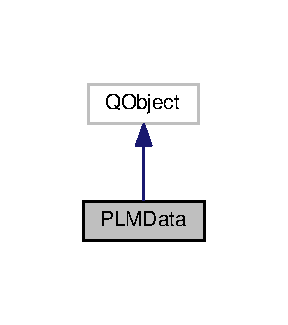
\includegraphics[width=138pt]{class_p_l_m_data__inherit__graph}
\end{center}
\end{figure}


Collaboration diagram for P\+L\+M\+Data\+:\nopagebreak
\begin{figure}[H]
\begin{center}
\leavevmode
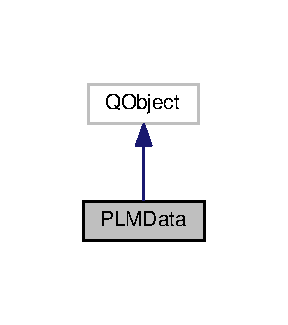
\includegraphics[width=138pt]{class_p_l_m_data__coll__graph}
\end{center}
\end{figure}
\subsection*{Public Member Functions}
\begin{DoxyCompactItemize}
\item 
{\bfseries P\+L\+M\+Data} (Q\+Object $\ast$parent=0)\hypertarget{class_p_l_m_data_abc3e70cb0be3ef1d02b01bc6a522e961}{}\label{class_p_l_m_data_abc3e70cb0be3ef1d02b01bc6a522e961}

\item 
\hyperlink{class_p_l_m_signal_hub}{P\+L\+M\+Signal\+Hub} $\ast$ {\bfseries signal\+Hub} ()\hypertarget{class_p_l_m_data_ad0be4ac0a80f670cef3dd15c95c4fad7}{}\label{class_p_l_m_data_ad0be4ac0a80f670cef3dd15c95c4fad7}

\item 
\hyperlink{class_p_l_m_error_hub}{P\+L\+M\+Error\+Hub} $\ast$ {\bfseries error\+Hub} ()\hypertarget{class_p_l_m_data_a9906f35dff1fe1185c6253fb1ff62704}{}\label{class_p_l_m_data_a9906f35dff1fe1185c6253fb1ff62704}

\item 
\hyperlink{class_p_l_m_write_hub}{P\+L\+M\+Write\+Hub} $\ast$ {\bfseries write\+Hub} ()\hypertarget{class_p_l_m_data_a761afe4ea6ddc308989ae2cb264ec7b2}{}\label{class_p_l_m_data_a761afe4ea6ddc308989ae2cb264ec7b2}

\item 
\hyperlink{class_p_l_m_project_hub}{P\+L\+M\+Project\+Hub} $\ast$ {\bfseries project\+Hub} ()\hypertarget{class_p_l_m_data_aab08c71ae40b351326e17df84c26f9be}{}\label{class_p_l_m_data_aab08c71ae40b351326e17df84c26f9be}

\end{DoxyCompactItemize}
\subsection*{Static Public Member Functions}
\begin{DoxyCompactItemize}
\item 
static \hyperlink{class_p_l_m_data}{P\+L\+M\+Data} $\ast$ {\bfseries instance} ()\hypertarget{class_p_l_m_data_ae73caded7d6db72017f21502b7089c4d}{}\label{class_p_l_m_data_ae73caded7d6db72017f21502b7089c4d}

\end{DoxyCompactItemize}


The documentation for this class was generated from the following files\+:\begin{DoxyCompactItemize}
\item 
src/plmdata.\+h\item 
src/plmdata.\+cpp\end{DoxyCompactItemize}

\hypertarget{struct_p_l_m_db_error}{}\section{P\+L\+M\+Db\+Error Struct Reference}
\label{struct_p_l_m_db_error}\index{P\+L\+M\+Db\+Error@{P\+L\+M\+Db\+Error}}
\subsection*{Public Types}
\begin{DoxyCompactItemize}
\item 
enum {\bfseries Return\+Error} \{ {\bfseries Error} =0, 
{\bfseries OK} =1
 \}\hypertarget{struct_p_l_m_db_error_aaf5ee57ca577a094f23cec1c195965cf}{}\label{struct_p_l_m_db_error_aaf5ee57ca577a094f23cec1c195965cf}

\item 
enum {\bfseries Error} \{ {\bfseries Invalid\+Type} =1, 
{\bfseries Invalid\+Parameter} =2, 
{\bfseries Internal\+Error} =3, 
{\bfseries Requested\+Record\+Not\+Found} =4
 \}\hypertarget{struct_p_l_m_db_error_a48e11f0b78e3a889668ecfe25d239402}{}\label{struct_p_l_m_db_error_a48e11f0b78e3a889668ecfe25d239402}

\end{DoxyCompactItemize}
\subsection*{Public Member Functions}
\begin{DoxyCompactItemize}
\item 
Q\+String {\bfseries get\+Status} () const \hypertarget{struct_p_l_m_db_error_af1eea58d11efb9e9d10867e41765997a}{}\label{struct_p_l_m_db_error_af1eea58d11efb9e9d10867e41765997a}

\item 
void {\bfseries set\+Status} (int status, int parameter, const Q\+String \&error\+Msg)\hypertarget{struct_p_l_m_db_error_a985a2a614d70453f86c84ffa0df2379a}{}\label{struct_p_l_m_db_error_a985a2a614d70453f86c84ffa0df2379a}

\end{DoxyCompactItemize}
\subsection*{Public Attributes}
\begin{DoxyCompactItemize}
\item 
int {\bfseries status}\hypertarget{struct_p_l_m_db_error_a2b258798884598e32ce5391ef4895f63}{}\label{struct_p_l_m_db_error_a2b258798884598e32ce5391ef4895f63}

\item 
int {\bfseries parameter}\hypertarget{struct_p_l_m_db_error_a347b0618011dfcdc200b235fd7265297}{}\label{struct_p_l_m_db_error_a347b0618011dfcdc200b235fd7265297}

\item 
Q\+String {\bfseries error\+Msg}\hypertarget{struct_p_l_m_db_error_ace09c3fafe8fa3974537c8182490f314}{}\label{struct_p_l_m_db_error_ace09c3fafe8fa3974537c8182490f314}

\end{DoxyCompactItemize}


The documentation for this struct was generated from the following file\+:\begin{DoxyCompactItemize}
\item 
src/tasks/sql/tree/plmdberror.\+h\end{DoxyCompactItemize}

\hypertarget{class_p_l_m_db_paper}{}\section{P\+L\+M\+Db\+Paper Class Reference}
\label{class_p_l_m_db_paper}\index{P\+L\+M\+Db\+Paper@{P\+L\+M\+Db\+Paper}}
\subsection*{Public Member Functions}
\begin{DoxyCompactItemize}
\item 
{\bfseries P\+L\+M\+Db\+Paper} (const Q\+Sql\+Database \&sql\+Db, const Q\+String \&table\+Name, const Q\+String \&id\+Name, int paper\+Id, bool commit)\hypertarget{class_p_l_m_db_paper_ae62948dc66edef1c6dab27a9c480dee7}{}\label{class_p_l_m_db_paper_ae62948dc66edef1c6dab27a9c480dee7}

\item 
bool {\bfseries get\+Commit} ()\hypertarget{class_p_l_m_db_paper_a9c2e66e0003109be3f6b9fabd34d78af}{}\label{class_p_l_m_db_paper_a9c2e66e0003109be3f6b9fabd34d78af}

\item 
void {\bfseries set\+Commit} (bool commit)\hypertarget{class_p_l_m_db_paper_ad76af3948288935278b0ac62f9cbfcb1}{}\label{class_p_l_m_db_paper_ad76af3948288935278b0ac62f9cbfcb1}

\item 
Q\+Variant {\bfseries get} (const Q\+String \&value\+Name) const \hypertarget{class_p_l_m_db_paper_aa33ba73641840a076e0740b561526c3a}{}\label{class_p_l_m_db_paper_aa33ba73641840a076e0740b561526c3a}

\item 
void {\bfseries set} (const Q\+String \&value\+Name, const Q\+Variant \&value)\hypertarget{class_p_l_m_db_paper_aedd3125b90e16706cd955485a1da08ea}{}\label{class_p_l_m_db_paper_aedd3125b90e16706cd955485a1da08ea}

\item 
int {\bfseries get\+Sort\+Order} ()\hypertarget{class_p_l_m_db_paper_a262348110b3a82d1d086a5d963937256}{}\label{class_p_l_m_db_paper_a262348110b3a82d1d086a5d963937256}

\item 
void {\bfseries set\+Sort\+Order} (int value)\hypertarget{class_p_l_m_db_paper_abc5d04213f6dbc76b12390de388c3757}{}\label{class_p_l_m_db_paper_abc5d04213f6dbc76b12390de388c3757}

\item 
int {\bfseries get\+Indent} ()\hypertarget{class_p_l_m_db_paper_a3252c61d00f31e6dae30a167cb03be00}{}\label{class_p_l_m_db_paper_a3252c61d00f31e6dae30a167cb03be00}

\item 
void {\bfseries set\+Indent} (int value)\hypertarget{class_p_l_m_db_paper_aa1e71597f038c5ecf392f18f1d1febf8}{}\label{class_p_l_m_db_paper_aa1e71597f038c5ecf392f18f1d1febf8}

\item 
Q\+Variant {\bfseries get\+Content} () const \hypertarget{class_p_l_m_db_paper_ad4e2542f29ceee25765777a57f808906}{}\label{class_p_l_m_db_paper_ad4e2542f29ceee25765777a57f808906}

\item 
void {\bfseries set\+Content} (const Q\+Variant \&value)\hypertarget{class_p_l_m_db_paper_a555d02ec899e1f27f0457720749c9cba}{}\label{class_p_l_m_db_paper_a555d02ec899e1f27f0457720749c9cba}

\item 
Q\+String {\bfseries get\+Title} () const \hypertarget{class_p_l_m_db_paper_a0d5fb9abf891e64d04126a1815d0162d}{}\label{class_p_l_m_db_paper_a0d5fb9abf891e64d04126a1815d0162d}

\item 
void {\bfseries set\+Title} (const Q\+String \&value)\hypertarget{class_p_l_m_db_paper_a5abd5c4760d8ce7e7569fa127d3fcf94}{}\label{class_p_l_m_db_paper_a5abd5c4760d8ce7e7569fa127d3fcf94}

\item 
bool {\bfseries get\+Delete} () const \hypertarget{class_p_l_m_db_paper_a5812d8a6ae7e204cc8f88cbfb4992aa2}{}\label{class_p_l_m_db_paper_a5812d8a6ae7e204cc8f88cbfb4992aa2}

\item 
void {\bfseries set\+Delete} (bool value)\hypertarget{class_p_l_m_db_paper_a296b49e1a52e361f25ded52bd9b06884}{}\label{class_p_l_m_db_paper_a296b49e1a52e361f25ded52bd9b06884}

\item 
int {\bfseries add} ()\hypertarget{class_p_l_m_db_paper_a387aff393fce92901937c306d5a14a27}{}\label{class_p_l_m_db_paper_a387aff393fce92901937c306d5a14a27}

\item 
Q\+List$<$ int $>$ {\bfseries child\+Id\+List} ()\hypertarget{class_p_l_m_db_paper_a4553b9bc043e4a07a42c46d3fa1449c1}{}\label{class_p_l_m_db_paper_a4553b9bc043e4a07a42c46d3fa1449c1}

\item 
bool {\bfseries exists} ()\hypertarget{class_p_l_m_db_paper_ab7b943731ea3823a7ea87c2a2f32149c}{}\label{class_p_l_m_db_paper_ab7b943731ea3823a7ea87c2a2f32149c}

\item 
int {\bfseries copy} (const Q\+String \&prefix)\hypertarget{class_p_l_m_db_paper_ab83ff7e669ff1f67278437b817922d13}{}\label{class_p_l_m_db_paper_ab83ff7e669ff1f67278437b817922d13}

\item 
void {\bfseries commit} ()\hypertarget{class_p_l_m_db_paper_a996ff074e3aa590de9646e2eb8a17f44}{}\label{class_p_l_m_db_paper_a996ff074e3aa590de9646e2eb8a17f44}

\item 
Q\+String \hyperlink{class_p_l_m_db_paper_a1dba36cb2bafff91d2e8a510d200ebe3}{get\+Last\+Executed\+Query} (const Q\+Sql\+Query \&query)
\begin{DoxyCompactList}\small\item\em get\+Last\+Executed\+Query \end{DoxyCompactList}\end{DoxyCompactItemize}


\subsection{Member Function Documentation}
\index{P\+L\+M\+Db\+Paper@{P\+L\+M\+Db\+Paper}!get\+Last\+Executed\+Query@{get\+Last\+Executed\+Query}}
\index{get\+Last\+Executed\+Query@{get\+Last\+Executed\+Query}!P\+L\+M\+Db\+Paper@{P\+L\+M\+Db\+Paper}}
\subsubsection[{\texorpdfstring{get\+Last\+Executed\+Query(const Q\+Sql\+Query \&query)}{getLastExecutedQuery(const QSqlQuery &query)}}]{\setlength{\rightskip}{0pt plus 5cm}Q\+String P\+L\+M\+Db\+Paper\+::get\+Last\+Executed\+Query (
\begin{DoxyParamCaption}
\item[{const Q\+Sql\+Query \&}]{query}
\end{DoxyParamCaption}
)\hspace{0.3cm}{\ttfamily [inline]}}\hypertarget{class_p_l_m_db_paper_a1dba36cb2bafff91d2e8a510d200ebe3}{}\label{class_p_l_m_db_paper_a1dba36cb2bafff91d2e8a510d200ebe3}


get\+Last\+Executed\+Query 


\begin{DoxyParams}{Parameters}
{\em query} & \\
\hline
\end{DoxyParams}
\begin{DoxyReturn}{Returns}
Useful for debugging 
\end{DoxyReturn}


The documentation for this class was generated from the following files\+:\begin{DoxyCompactItemize}
\item 
src/tasks/sql/tree/plmdbpaper.\+h\item 
src/tasks/sql/tree/plmdbpaper.\+cpp\end{DoxyCompactItemize}

\hypertarget{class_p_l_m_db_tree}{}\section{P\+L\+M\+Db\+Tree Class Reference}
\label{class_p_l_m_db_tree}\index{P\+L\+M\+Db\+Tree@{P\+L\+M\+Db\+Tree}}
\subsection*{Public Member Functions}
\begin{DoxyCompactItemize}
\item 
\hyperlink{class_p_l_m_db_tree_a23d35341defc8ccd6cd75989eecca77b}{P\+L\+M\+Db\+Tree} (const Q\+Sql\+Database \&sql\+Db, const Q\+String \&table\+Name, const Q\+String \&id\+Name, bool commit)
\begin{DoxyCompactList}\small\item\em \hyperlink{class_p_l_m_db_tree_a23d35341defc8ccd6cd75989eecca77b}{P\+L\+M\+Db\+Tree\+::\+P\+L\+M\+Db\+Tree}. \end{DoxyCompactList}\item 
void \hyperlink{class_p_l_m_db_tree_aeab32bcea9b1ff524eeefa34248a5d86}{set\+Commit} (bool value)
\begin{DoxyCompactList}\small\item\em \hyperlink{class_p_l_m_db_tree_aeab32bcea9b1ff524eeefa34248a5d86}{P\+L\+M\+Db\+Tree\+::set\+Commit}. \end{DoxyCompactList}\item 
bool \hyperlink{class_p_l_m_db_tree_a68299ded7c927c8c2557915811ac9d10}{get\+Commit} ()
\begin{DoxyCompactList}\small\item\em \hyperlink{class_p_l_m_db_tree_a68299ded7c927c8c2557915811ac9d10}{P\+L\+M\+Db\+Tree\+::get\+Commit}. \end{DoxyCompactList}\item 
void \hyperlink{class_p_l_m_db_tree_a0ac15c9ac8b51d15c20ab6b7f03e60cb}{renum\+All} ()\hypertarget{class_p_l_m_db_tree_a0ac15c9ac8b51d15c20ab6b7f03e60cb}{}\label{class_p_l_m_db_tree_a0ac15c9ac8b51d15c20ab6b7f03e60cb}

\begin{DoxyCompactList}\small\item\em \hyperlink{class_p_l_m_db_tree_a0ac15c9ac8b51d15c20ab6b7f03e60cb}{P\+L\+M\+Db\+Tree\+::renum\+All}. \end{DoxyCompactList}\item 
\hyperlink{struct_p_l_m_db_error}{P\+L\+M\+Db\+Error} {\bfseries error} ()\hypertarget{class_p_l_m_db_tree_ad42a344bcf5101bf5d8456f390185476}{}\label{class_p_l_m_db_tree_ad42a344bcf5101bf5d8456f390185476}

\item 
int \hyperlink{class_p_l_m_db_tree_aec9236c55a24d2bae0ee26a5f78b55a2}{move\+List} (Q\+List$<$ int $>$ id\+List, int paper\+Id)
\begin{DoxyCompactList}\small\item\em \hyperlink{class_p_l_m_db_tree_aec9236c55a24d2bae0ee26a5f78b55a2}{P\+L\+M\+Db\+Tree\+::move\+List}. \end{DoxyCompactList}\item 
int \hyperlink{class_p_l_m_db_tree_aeaa59f400d18e4b299ee4b64bd0755d0}{copy\+List} (Q\+List$<$ int $>$ id\+List)
\begin{DoxyCompactList}\small\item\em \hyperlink{class_p_l_m_db_tree_aeaa59f400d18e4b299ee4b64bd0755d0}{P\+L\+M\+Db\+Tree\+::copy\+List}. \end{DoxyCompactList}\item 
int {\bfseries delete\+List} (Q\+List$<$ int $>$ id\+List)\hypertarget{class_p_l_m_db_tree_ab3adc738f0f85176c9683e50a45c56cf}{}\label{class_p_l_m_db_tree_ab3adc738f0f85176c9683e50a45c56cf}

\item 
int {\bfseries undelete\+List} (Q\+List$<$ int $>$ id\+List)\hypertarget{class_p_l_m_db_tree_a38c4400623873f8fb0c4e7e93d192fd5}{}\label{class_p_l_m_db_tree_a38c4400623873f8fb0c4e7e93d192fd5}

\item 
int {\bfseries empty\+Trash} ()\hypertarget{class_p_l_m_db_tree_a85022035f9a223c3299f56302c60e637}{}\label{class_p_l_m_db_tree_a85022035f9a223c3299f56302c60e637}

\item 
Q\+List$<$ int $>$ {\bfseries list\+Visible\+Id} ()\hypertarget{class_p_l_m_db_tree_a997d67ba34d62868e94411b226e8477b}{}\label{class_p_l_m_db_tree_a997d67ba34d62868e94411b226e8477b}

\item 
Q\+List$<$ int $>$ {\bfseries list\+Trash} ()\hypertarget{class_p_l_m_db_tree_a7ba474277585d6fd8af2eda724ca381c}{}\label{class_p_l_m_db_tree_a7ba474277585d6fd8af2eda724ca381c}

\item 
Q\+List$<$ int $>$ {\bfseries list\+All} ()\hypertarget{class_p_l_m_db_tree_a993d122fd1c2da3920ceaaccb14fe713}{}\label{class_p_l_m_db_tree_a993d122fd1c2da3920ceaaccb14fe713}

\item 
int {\bfseries get\+Paper\+Above} (int paper\+Id)\hypertarget{class_p_l_m_db_tree_a6c9df6e19f061259cffc41bf5e85a0bc}{}\label{class_p_l_m_db_tree_a6c9df6e19f061259cffc41bf5e85a0bc}

\item 
int {\bfseries get\+Paper\+Below} (int paper\+Id)\hypertarget{class_p_l_m_db_tree_a7156ec828975d56f3d18aead75cd8e0c}{}\label{class_p_l_m_db_tree_a7156ec828975d56f3d18aead75cd8e0c}

\item 
Q\+String {\bfseries get\+Last\+Executed\+Query} (const Q\+Sql\+Query \&query)\hypertarget{class_p_l_m_db_tree_a14ea98b38d2c88d97f22ad97f808fdd2}{}\label{class_p_l_m_db_tree_a14ea98b38d2c88d97f22ad97f808fdd2}

\end{DoxyCompactItemize}


\subsection{Constructor \& Destructor Documentation}
\index{P\+L\+M\+Db\+Tree@{P\+L\+M\+Db\+Tree}!P\+L\+M\+Db\+Tree@{P\+L\+M\+Db\+Tree}}
\index{P\+L\+M\+Db\+Tree@{P\+L\+M\+Db\+Tree}!P\+L\+M\+Db\+Tree@{P\+L\+M\+Db\+Tree}}
\subsubsection[{\texorpdfstring{P\+L\+M\+Db\+Tree(const Q\+Sql\+Database \&sql\+Db, const Q\+String \&table\+Name, const Q\+String \&id\+Name, bool commit)}{PLMDbTree(const QSqlDatabase &sqlDb, const QString &tableName, const QString &idName, bool commit)}}]{\setlength{\rightskip}{0pt plus 5cm}P\+L\+M\+Db\+Tree\+::\+P\+L\+M\+Db\+Tree (
\begin{DoxyParamCaption}
\item[{const Q\+Sql\+Database \&}]{sql\+Db, }
\item[{const Q\+String \&}]{table\+Name, }
\item[{const Q\+String \&}]{id\+Name, }
\item[{bool}]{commit}
\end{DoxyParamCaption}
)}\hypertarget{class_p_l_m_db_tree_a23d35341defc8ccd6cd75989eecca77b}{}\label{class_p_l_m_db_tree_a23d35341defc8ccd6cd75989eecca77b}


\hyperlink{class_p_l_m_db_tree_a23d35341defc8ccd6cd75989eecca77b}{P\+L\+M\+Db\+Tree\+::\+P\+L\+M\+Db\+Tree}. 


\begin{DoxyParams}{Parameters}
{\em sql\+Db} & \\
\hline
{\em table\+Name} & \\
\hline
{\em id\+Name} & \\
\hline
{\em commit} & \\
\hline
\end{DoxyParams}


\subsection{Member Function Documentation}
\index{P\+L\+M\+Db\+Tree@{P\+L\+M\+Db\+Tree}!copy\+List@{copy\+List}}
\index{copy\+List@{copy\+List}!P\+L\+M\+Db\+Tree@{P\+L\+M\+Db\+Tree}}
\subsubsection[{\texorpdfstring{copy\+List(\+Q\+List$<$ int $>$ id\+List)}{copyList(QList< int > idList)}}]{\setlength{\rightskip}{0pt plus 5cm}int P\+L\+M\+Db\+Tree\+::copy\+List (
\begin{DoxyParamCaption}
\item[{Q\+List$<$ int $>$}]{id\+List}
\end{DoxyParamCaption}
)}\hypertarget{class_p_l_m_db_tree_aeaa59f400d18e4b299ee4b64bd0755d0}{}\label{class_p_l_m_db_tree_aeaa59f400d18e4b299ee4b64bd0755d0}


\hyperlink{class_p_l_m_db_tree_aeaa59f400d18e4b299ee4b64bd0755d0}{P\+L\+M\+Db\+Tree\+::copy\+List}. 


\begin{DoxyParams}{Parameters}
{\em id\+List} & \\
\hline
\end{DoxyParams}
\begin{DoxyReturn}{Returns}

\end{DoxyReturn}
\index{P\+L\+M\+Db\+Tree@{P\+L\+M\+Db\+Tree}!get\+Commit@{get\+Commit}}
\index{get\+Commit@{get\+Commit}!P\+L\+M\+Db\+Tree@{P\+L\+M\+Db\+Tree}}
\subsubsection[{\texorpdfstring{get\+Commit()}{getCommit()}}]{\setlength{\rightskip}{0pt plus 5cm}bool P\+L\+M\+Db\+Tree\+::get\+Commit (
\begin{DoxyParamCaption}
{}
\end{DoxyParamCaption}
)}\hypertarget{class_p_l_m_db_tree_a68299ded7c927c8c2557915811ac9d10}{}\label{class_p_l_m_db_tree_a68299ded7c927c8c2557915811ac9d10}


\hyperlink{class_p_l_m_db_tree_a68299ded7c927c8c2557915811ac9d10}{P\+L\+M\+Db\+Tree\+::get\+Commit}. 

\begin{DoxyReturn}{Returns}

\end{DoxyReturn}
\index{P\+L\+M\+Db\+Tree@{P\+L\+M\+Db\+Tree}!move\+List@{move\+List}}
\index{move\+List@{move\+List}!P\+L\+M\+Db\+Tree@{P\+L\+M\+Db\+Tree}}
\subsubsection[{\texorpdfstring{move\+List(\+Q\+List$<$ int $>$ id\+List, int paper\+Id)}{moveList(QList< int > idList, int paperId)}}]{\setlength{\rightskip}{0pt plus 5cm}int P\+L\+M\+Db\+Tree\+::move\+List (
\begin{DoxyParamCaption}
\item[{Q\+List$<$ int $>$}]{id\+List, }
\item[{int}]{paper\+Id}
\end{DoxyParamCaption}
)}\hypertarget{class_p_l_m_db_tree_aec9236c55a24d2bae0ee26a5f78b55a2}{}\label{class_p_l_m_db_tree_aec9236c55a24d2bae0ee26a5f78b55a2}


\hyperlink{class_p_l_m_db_tree_aec9236c55a24d2bae0ee26a5f78b55a2}{P\+L\+M\+Db\+Tree\+::move\+List}. 


\begin{DoxyParams}{Parameters}
{\em id\+List} & \\
\hline
{\em paper\+Id} & \\
\hline
\end{DoxyParams}
\begin{DoxyReturn}{Returns}

\end{DoxyReturn}
\index{P\+L\+M\+Db\+Tree@{P\+L\+M\+Db\+Tree}!set\+Commit@{set\+Commit}}
\index{set\+Commit@{set\+Commit}!P\+L\+M\+Db\+Tree@{P\+L\+M\+Db\+Tree}}
\subsubsection[{\texorpdfstring{set\+Commit(bool value)}{setCommit(bool value)}}]{\setlength{\rightskip}{0pt plus 5cm}void P\+L\+M\+Db\+Tree\+::set\+Commit (
\begin{DoxyParamCaption}
\item[{bool}]{value}
\end{DoxyParamCaption}
)}\hypertarget{class_p_l_m_db_tree_aeab32bcea9b1ff524eeefa34248a5d86}{}\label{class_p_l_m_db_tree_aeab32bcea9b1ff524eeefa34248a5d86}


\hyperlink{class_p_l_m_db_tree_aeab32bcea9b1ff524eeefa34248a5d86}{P\+L\+M\+Db\+Tree\+::set\+Commit}. 


\begin{DoxyParams}{Parameters}
{\em value} & \\
\hline
\end{DoxyParams}


The documentation for this class was generated from the following files\+:\begin{DoxyCompactItemize}
\item 
src/tasks/sql/tree/plmdbtree.\+h\item 
src/tasks/sql/tree/plmdbtree.\+cpp\end{DoxyCompactItemize}

\hypertarget{struct_p_l_m_error}{}\section{P\+L\+M\+Error Struct Reference}
\label{struct_p_l_m_error}\index{P\+L\+M\+Error@{P\+L\+M\+Error}}
\subsection*{Public Member Functions}
\begin{DoxyCompactItemize}
\item 
{\bfseries P\+L\+M\+Error} (const Q\+String \&\+\_\+error\+Code, const Q\+String \&\+\_\+origin, const Q\+String \&\+\_\+message)\hypertarget{struct_p_l_m_error_a1c7506dd5f92e0fc5623e69913d1e1dc}{}\label{struct_p_l_m_error_a1c7506dd5f92e0fc5623e69913d1e1dc}

\item 
{\bfseries P\+L\+M\+Error} (const \hyperlink{struct_p_l_m_error}{P\+L\+M\+Error} \&other)\hypertarget{struct_p_l_m_error_ab3452bc2a78eb5703c6275f75ac58f08}{}\label{struct_p_l_m_error_ab3452bc2a78eb5703c6275f75ac58f08}

\item 
Q\+String {\bfseries error\+Code} () const \hypertarget{struct_p_l_m_error_a92c888b245c56159ed52a7b62499e05a}{}\label{struct_p_l_m_error_a92c888b245c56159ed52a7b62499e05a}

\item 
Q\+String {\bfseries origin} () const \hypertarget{struct_p_l_m_error_a2d83f9bd2c2f4ae3e50ab69385f7b943}{}\label{struct_p_l_m_error_a2d83f9bd2c2f4ae3e50ab69385f7b943}

\item 
Q\+String {\bfseries message} () const \hypertarget{struct_p_l_m_error_a070e473664207f3b31eaf52f2a419aa5}{}\label{struct_p_l_m_error_a070e473664207f3b31eaf52f2a419aa5}

\item 
Q\+List$<$ Q\+String $>$ {\bfseries get\+All} () const \hypertarget{struct_p_l_m_error_a3be7c3f7778f48f785c2607c6b13174a}{}\label{struct_p_l_m_error_a3be7c3f7778f48f785c2607c6b13174a}

\end{DoxyCompactItemize}


The documentation for this struct was generated from the following file\+:\begin{DoxyCompactItemize}
\item 
src/plmerrorhub.\+h\end{DoxyCompactItemize}

\hypertarget{class_p_l_m_error_hub}{}\section{P\+L\+M\+Error\+Hub Class Reference}
\label{class_p_l_m_error_hub}\index{P\+L\+M\+Error\+Hub@{P\+L\+M\+Error\+Hub}}


Inheritance diagram for P\+L\+M\+Error\+Hub\+:\nopagebreak
\begin{figure}[H]
\begin{center}
\leavevmode
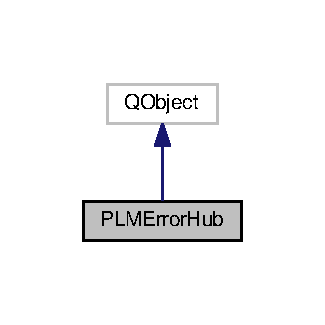
\includegraphics[width=156pt]{class_p_l_m_error_hub__inherit__graph}
\end{center}
\end{figure}


Collaboration diagram for P\+L\+M\+Error\+Hub\+:\nopagebreak
\begin{figure}[H]
\begin{center}
\leavevmode
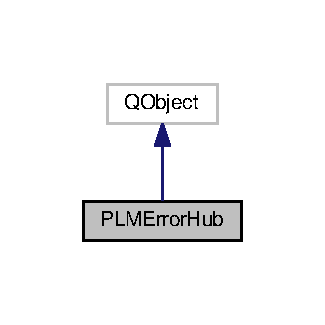
\includegraphics[width=156pt]{class_p_l_m_error_hub__coll__graph}
\end{center}
\end{figure}
\subsection*{Public Slots}
\begin{DoxyCompactItemize}
\item 
void {\bfseries add\+Error} (const Q\+String \&error\+Code, const Q\+String \&origin, const Q\+String \&message)\hypertarget{class_p_l_m_error_hub_a79bcc021f473fbbd695970a871383d46}{}\label{class_p_l_m_error_hub_a79bcc021f473fbbd695970a871383d46}

\end{DoxyCompactItemize}
\subsection*{Signals}
\begin{DoxyCompactItemize}
\item 
void {\bfseries error\+Sent} (const Q\+String \&error\+Code, const Q\+String \&origin, const Q\+String \&message)\hypertarget{class_p_l_m_error_hub_ac6fbc995d2278d6770d1fede0a55c811}{}\label{class_p_l_m_error_hub_ac6fbc995d2278d6770d1fede0a55c811}

\item 
void {\bfseries error\+Sent} ()\hypertarget{class_p_l_m_error_hub_ae88787d18851112cc459cebc3485d8a9}{}\label{class_p_l_m_error_hub_ae88787d18851112cc459cebc3485d8a9}

\end{DoxyCompactItemize}
\subsection*{Public Member Functions}
\begin{DoxyCompactItemize}
\item 
{\bfseries P\+L\+M\+Error\+Hub} (Q\+Object $\ast$parent)\hypertarget{class_p_l_m_error_hub_a52e272cb8c0ae4a1e8c57b34fafb0d85}{}\label{class_p_l_m_error_hub_a52e272cb8c0ae4a1e8c57b34fafb0d85}

\item 
Q\+List$<$ Q\+String $>$ {\bfseries getlatest\+Error} () const \hypertarget{class_p_l_m_error_hub_a12aa63f7e81db43b7ba2644b6611f5e7}{}\label{class_p_l_m_error_hub_a12aa63f7e81db43b7ba2644b6611f5e7}

\item 
Q\+List$<$ Q\+String $>$ {\bfseries get\+Error} (int index) const \hypertarget{class_p_l_m_error_hub_ade5b6fcd2db59f8a515748b9f8fac109}{}\label{class_p_l_m_error_hub_ade5b6fcd2db59f8a515748b9f8fac109}

\item 
int {\bfseries count} ()\hypertarget{class_p_l_m_error_hub_a65a23a53f162183bdb5359069dfdeaa4}{}\label{class_p_l_m_error_hub_a65a23a53f162183bdb5359069dfdeaa4}

\item 
void {\bfseries clear} ()\hypertarget{class_p_l_m_error_hub_a5858e0f97f67f182e76a6b5a76e57444}{}\label{class_p_l_m_error_hub_a5858e0f97f67f182e76a6b5a76e57444}

\end{DoxyCompactItemize}


The documentation for this class was generated from the following files\+:\begin{DoxyCompactItemize}
\item 
src/plmerrorhub.\+h\item 
src/plmerrorhub.\+cpp\end{DoxyCompactItemize}

\hypertarget{class_p_l_m_exporter}{}\section{P\+L\+M\+Exporter Class Reference}
\label{class_p_l_m_exporter}\index{P\+L\+M\+Exporter@{P\+L\+M\+Exporter}}


Inheritance diagram for P\+L\+M\+Exporter\+:\nopagebreak
\begin{figure}[H]
\begin{center}
\leavevmode
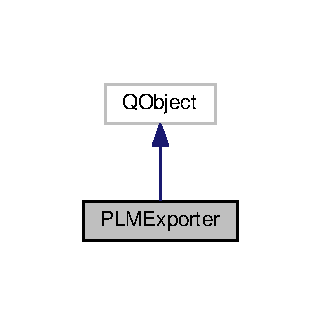
\includegraphics[width=154pt]{class_p_l_m_exporter__inherit__graph}
\end{center}
\end{figure}


Collaboration diagram for P\+L\+M\+Exporter\+:\nopagebreak
\begin{figure}[H]
\begin{center}
\leavevmode
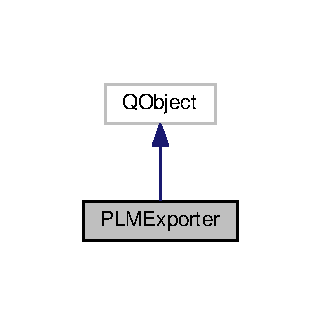
\includegraphics[width=154pt]{class_p_l_m_exporter__coll__graph}
\end{center}
\end{figure}
\subsection*{Public Member Functions}
\begin{DoxyCompactItemize}
\item 
{\bfseries P\+L\+M\+Exporter} (Q\+Object $\ast$parent=0)\hypertarget{class_p_l_m_exporter_ae43f6456a8e870c309704bbd78d7c6ca}{}\label{class_p_l_m_exporter_ae43f6456a8e870c309704bbd78d7c6ca}

\end{DoxyCompactItemize}
\subsection*{Static Public Member Functions}
\begin{DoxyCompactItemize}
\item 
static bool {\bfseries export\+S\+Q\+Lite\+Db\+To} (\hyperlink{class_p_l_m_project}{P\+L\+M\+Project} $\ast$db, const Q\+String \&type, const Q\+String \&file\+Name)\hypertarget{class_p_l_m_exporter_a69d82f803a8f20cd47ed4a0c80ad7f84}{}\label{class_p_l_m_exporter_a69d82f803a8f20cd47ed4a0c80ad7f84}

\end{DoxyCompactItemize}


The documentation for this class was generated from the following files\+:\begin{DoxyCompactItemize}
\item 
src/tasks/sql/plmexporter.\+h\item 
src/tasks/sql/plmexporter.\+cpp\end{DoxyCompactItemize}

\hypertarget{class_p_l_m_importer}{}\section{P\+L\+M\+Importer Class Reference}
\label{class_p_l_m_importer}\index{P\+L\+M\+Importer@{P\+L\+M\+Importer}}


Inheritance diagram for P\+L\+M\+Importer\+:\nopagebreak
\begin{figure}[H]
\begin{center}
\leavevmode
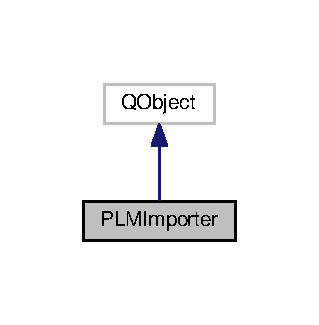
\includegraphics[width=153pt]{class_p_l_m_importer__inherit__graph}
\end{center}
\end{figure}


Collaboration diagram for P\+L\+M\+Importer\+:\nopagebreak
\begin{figure}[H]
\begin{center}
\leavevmode
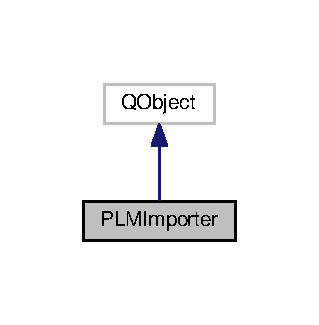
\includegraphics[width=153pt]{class_p_l_m_importer__coll__graph}
\end{center}
\end{figure}
\subsection*{Public Member Functions}
\begin{DoxyCompactItemize}
\item 
{\bfseries P\+L\+M\+Importer} (Q\+Object $\ast$parent=0)\hypertarget{class_p_l_m_importer_abe28800196747217ddeb78cc463de130}{}\label{class_p_l_m_importer_abe28800196747217ddeb78cc463de130}

\item 
Q\+Sql\+Database {\bfseries create\+S\+Q\+Lite\+Db\+From} (const Q\+String \&type, const Q\+String \&file\+Name, int project\+Id)\hypertarget{class_p_l_m_importer_aaaefaf1e4e123361b47e815381694727}{}\label{class_p_l_m_importer_aaaefaf1e4e123361b47e815381694727}

\item 
Q\+Sql\+Database {\bfseries create\+Empty\+S\+Q\+Lite\+Project} (int project\+Id)\hypertarget{class_p_l_m_importer_a884a8b0e0341243cb02654d08d99f4d0}{}\label{class_p_l_m_importer_a884a8b0e0341243cb02654d08d99f4d0}

\end{DoxyCompactItemize}


The documentation for this class was generated from the following files\+:\begin{DoxyCompactItemize}
\item 
src/tasks/sql/plmimporter.\+h\item 
src/tasks/sql/plmimporter.\+cpp\end{DoxyCompactItemize}

\hypertarget{class_p_l_m_note_tree}{}\section{P\+L\+M\+Note\+Tree Class Reference}
\label{class_p_l_m_note_tree}\index{P\+L\+M\+Note\+Tree@{P\+L\+M\+Note\+Tree}}


Inheritance diagram for P\+L\+M\+Note\+Tree\+:\nopagebreak
\begin{figure}[H]
\begin{center}
\leavevmode
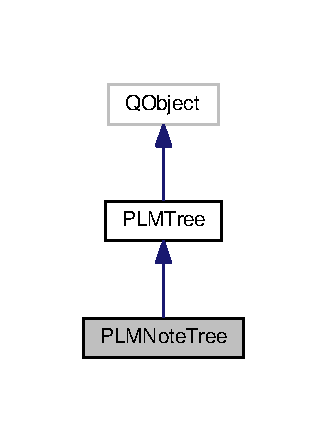
\includegraphics[width=157pt]{class_p_l_m_note_tree__inherit__graph}
\end{center}
\end{figure}


Collaboration diagram for P\+L\+M\+Note\+Tree\+:\nopagebreak
\begin{figure}[H]
\begin{center}
\leavevmode
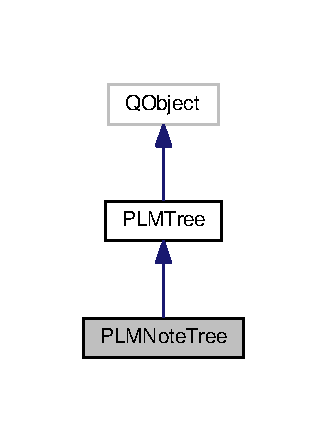
\includegraphics[width=157pt]{class_p_l_m_note_tree__coll__graph}
\end{center}
\end{figure}
\subsection*{Public Member Functions}
\begin{DoxyCompactItemize}
\item 
{\bfseries P\+L\+M\+Note\+Tree} (Q\+Object $\ast$parent, const Q\+String \&table\+Name, const Q\+String \&code\+Name, Q\+Sql\+Database sql\+Db)\hypertarget{class_p_l_m_note_tree_aa395393799f5b8fbb0cf6aa531ad7b13}{}\label{class_p_l_m_note_tree_aa395393799f5b8fbb0cf6aa531ad7b13}

\item 
int {\bfseries add\+New\+Child\+Note} (int parent\+Note\+Id=-\/1)\hypertarget{class_p_l_m_note_tree_ab6ac0c7604d9017cc2c20cf94da35b90}{}\label{class_p_l_m_note_tree_ab6ac0c7604d9017cc2c20cf94da35b90}

\item 
void {\bfseries move\+Note\+To\+Synopsis} (int parent\+Note\+Id)\hypertarget{class_p_l_m_note_tree_a448f0356af7b2cb17e038959423aa800}{}\label{class_p_l_m_note_tree_a448f0356af7b2cb17e038959423aa800}

\item 
bool {\bfseries get\+Is\+Synopsis} (int note\+Id)\hypertarget{class_p_l_m_note_tree_ab4a572fb6142f7a1ffdaf3885883351a}{}\label{class_p_l_m_note_tree_ab4a572fb6142f7a1ffdaf3885883351a}

\item 
void {\bfseries set\+Is\+Synopsis} (int note\+Id, bool value)\hypertarget{class_p_l_m_note_tree_a0cb70c674930a4b0bebb4532a0737aa0}{}\label{class_p_l_m_note_tree_a0cb70c674930a4b0bebb4532a0737aa0}

\item 
int {\bfseries get\+Sheet\+Code} (int note\+Id)\hypertarget{class_p_l_m_note_tree_a8355d84fa27bdaa0355c8be065372178}{}\label{class_p_l_m_note_tree_a8355d84fa27bdaa0355c8be065372178}

\item 
void {\bfseries set\+Sheet\+Code} (int note\+Id, int value)\hypertarget{class_p_l_m_note_tree_a90b6d91a8696286c42f77c83b3601de9}{}\label{class_p_l_m_note_tree_a90b6d91a8696286c42f77c83b3601de9}

\end{DoxyCompactItemize}
\subsection*{Additional Inherited Members}


The documentation for this class was generated from the following files\+:\begin{DoxyCompactItemize}
\item 
src/tasks/sql/tree/plmnotetree.\+h\item 
src/tasks/sql/tree/plmnotetree.\+cpp\end{DoxyCompactItemize}

\hypertarget{class_p_l_m_project}{}\section{P\+L\+M\+Project Class Reference}
\label{class_p_l_m_project}\index{P\+L\+M\+Project@{P\+L\+M\+Project}}


Inheritance diagram for P\+L\+M\+Project\+:\nopagebreak
\begin{figure}[H]
\begin{center}
\leavevmode
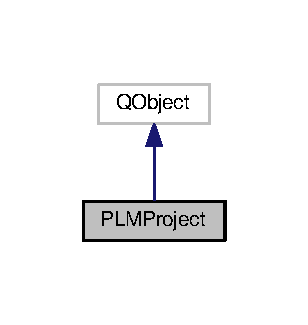
\includegraphics[width=148pt]{class_p_l_m_project__inherit__graph}
\end{center}
\end{figure}


Collaboration diagram for P\+L\+M\+Project\+:\nopagebreak
\begin{figure}[H]
\begin{center}
\leavevmode
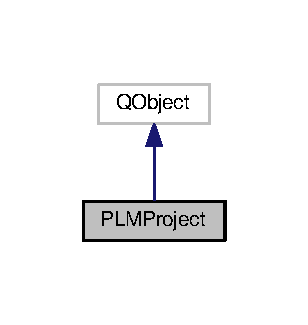
\includegraphics[width=148pt]{class_p_l_m_project__coll__graph}
\end{center}
\end{figure}
\subsection*{Public Slots}
\begin{DoxyCompactItemize}
\item 
void {\bfseries close} ()\hypertarget{class_p_l_m_project_a4134c6837f7a115582c18c2ef495ef83}{}\label{class_p_l_m_project_a4134c6837f7a115582c18c2ef495ef83}

\end{DoxyCompactItemize}
\subsection*{Public Member Functions}
\begin{DoxyCompactItemize}
\item 
{\bfseries P\+L\+M\+Project} (Q\+Object $\ast$parent, int project\+Id, const Q\+String \&file\+Name)\hypertarget{class_p_l_m_project_aea4d4bc12ab91752c2e5bab017f0ac82}{}\label{class_p_l_m_project_aea4d4bc12ab91752c2e5bab017f0ac82}

\item 
\hyperlink{class_p_l_m_property}{P\+L\+M\+Property} $\ast$ {\bfseries get\+Property} (const Q\+String \&table\+Name)\hypertarget{class_p_l_m_project_a0a55163d106463983a9d6cc4211f0a76}{}\label{class_p_l_m_project_a0a55163d106463983a9d6cc4211f0a76}

\item 
\hyperlink{class_p_l_m_tree}{P\+L\+M\+Tree} $\ast$ {\bfseries get\+Tree} (const Q\+String \&table\+Name)\hypertarget{class_p_l_m_project_a1a8c835fccc0c815635bd15bbde5b593}{}\label{class_p_l_m_project_a1a8c835fccc0c815635bd15bbde5b593}

\item 
\hyperlink{class_p_l_m_sheet_tree}{P\+L\+M\+Sheet\+Tree} $\ast$ {\bfseries sheet\+Tree} ()\hypertarget{class_p_l_m_project_ae8154e108519c03653e931db60c5aa85}{}\label{class_p_l_m_project_ae8154e108519c03653e931db60c5aa85}

\item 
\hyperlink{class_p_l_m_note_tree}{P\+L\+M\+Note\+Tree} $\ast$ {\bfseries note\+Tree} ()\hypertarget{class_p_l_m_project_a556db2493d0941ca4b942d9d4d5a3706}{}\label{class_p_l_m_project_a556db2493d0941ca4b942d9d4d5a3706}

\item 
Q\+String {\bfseries get\+Type} () const \hypertarget{class_p_l_m_project_a46a7edd0080785ffd078b607f007b17a}{}\label{class_p_l_m_project_a46a7edd0080785ffd078b607f007b17a}

\item 
void {\bfseries set\+Type} (const Q\+String \&value)\hypertarget{class_p_l_m_project_a682098f2b06e28d0eef4a6d1b002385b}{}\label{class_p_l_m_project_a682098f2b06e28d0eef4a6d1b002385b}

\item 
Q\+String {\bfseries get\+Temp\+File\+Name} () const \hypertarget{class_p_l_m_project_aba1306178d23255800a9e52709dbfd13}{}\label{class_p_l_m_project_aba1306178d23255800a9e52709dbfd13}

\end{DoxyCompactItemize}


The documentation for this class was generated from the following files\+:\begin{DoxyCompactItemize}
\item 
src/tasks/sql/plmproject.\+h\item 
src/tasks/sql/plmproject.\+cpp\end{DoxyCompactItemize}

\hypertarget{class_p_l_m_project_close_all_projects}{}\section{P\+L\+M\+Project\+Close\+All\+Projects Class Reference}
\label{class_p_l_m_project_close_all_projects}\index{P\+L\+M\+Project\+Close\+All\+Projects@{P\+L\+M\+Project\+Close\+All\+Projects}}


Inheritance diagram for P\+L\+M\+Project\+Close\+All\+Projects\+:\nopagebreak
\begin{figure}[H]
\begin{center}
\leavevmode
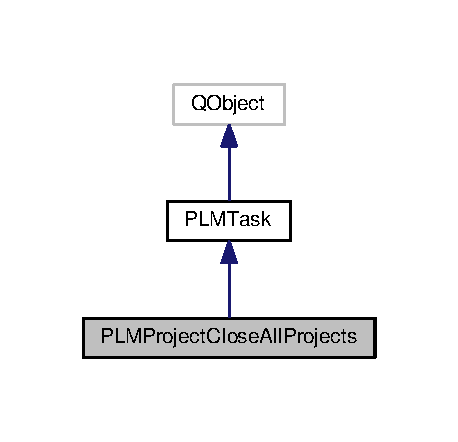
\includegraphics[width=220pt]{class_p_l_m_project_close_all_projects__inherit__graph}
\end{center}
\end{figure}


Collaboration diagram for P\+L\+M\+Project\+Close\+All\+Projects\+:\nopagebreak
\begin{figure}[H]
\begin{center}
\leavevmode
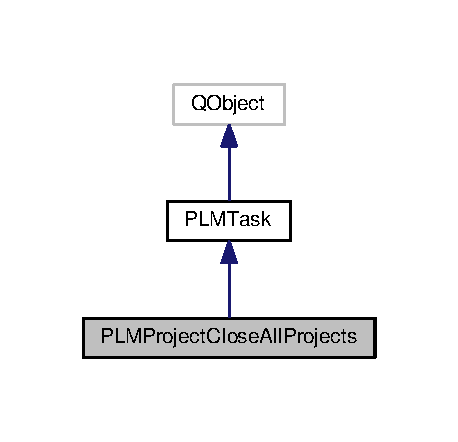
\includegraphics[width=220pt]{class_p_l_m_project_close_all_projects__coll__graph}
\end{center}
\end{figure}
\subsection*{Public Member Functions}
\begin{DoxyCompactItemize}
\item 
void {\bfseries do\+Task} (bool $\ast$ok)\hypertarget{class_p_l_m_project_close_all_projects_a47e3bc0cef4683806cddd7958305831d}{}\label{class_p_l_m_project_close_all_projects_a47e3bc0cef4683806cddd7958305831d}

\end{DoxyCompactItemize}
\subsection*{Additional Inherited Members}


The documentation for this class was generated from the following file\+:\begin{DoxyCompactItemize}
\item 
src/tasks/plmprojectcloseallprojects.\+h\end{DoxyCompactItemize}

\hypertarget{class_p_l_m_project_close_project}{}\section{P\+L\+M\+Project\+Close\+Project Class Reference}
\label{class_p_l_m_project_close_project}\index{P\+L\+M\+Project\+Close\+Project@{P\+L\+M\+Project\+Close\+Project}}


Inheritance diagram for P\+L\+M\+Project\+Close\+Project\+:\nopagebreak
\begin{figure}[H]
\begin{center}
\leavevmode
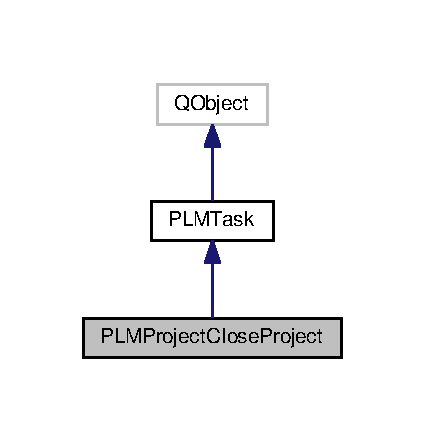
\includegraphics[width=204pt]{class_p_l_m_project_close_project__inherit__graph}
\end{center}
\end{figure}


Collaboration diagram for P\+L\+M\+Project\+Close\+Project\+:\nopagebreak
\begin{figure}[H]
\begin{center}
\leavevmode
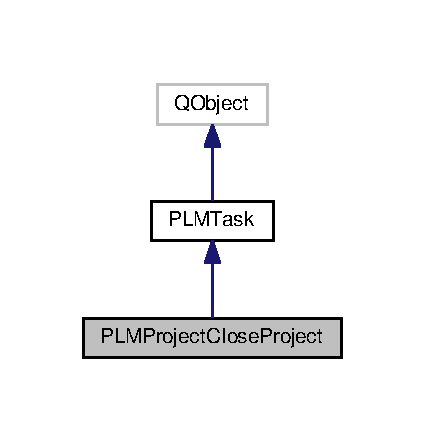
\includegraphics[width=204pt]{class_p_l_m_project_close_project__coll__graph}
\end{center}
\end{figure}
\subsection*{Public Member Functions}
\begin{DoxyCompactItemize}
\item 
{\bfseries P\+L\+M\+Project\+Close\+Project} (int project\+Id)\hypertarget{class_p_l_m_project_close_project_a08c831497553d51b64bce730d2d8c9a8}{}\label{class_p_l_m_project_close_project_a08c831497553d51b64bce730d2d8c9a8}

\item 
void {\bfseries do\+Task} (bool $\ast$ok)\hypertarget{class_p_l_m_project_close_project_aefc50afc81794804564e268f109e7b29}{}\label{class_p_l_m_project_close_project_aefc50afc81794804564e268f109e7b29}

\end{DoxyCompactItemize}
\subsection*{Additional Inherited Members}


The documentation for this class was generated from the following file\+:\begin{DoxyCompactItemize}
\item 
src/tasks/plmprojectcloseproject.\+h\end{DoxyCompactItemize}

\hypertarget{class_p_l_m_project_get_project_id_list}{}\section{P\+L\+M\+Project\+Get\+Project\+Id\+List Class Reference}
\label{class_p_l_m_project_get_project_id_list}\index{P\+L\+M\+Project\+Get\+Project\+Id\+List@{P\+L\+M\+Project\+Get\+Project\+Id\+List}}


Inheritance diagram for P\+L\+M\+Project\+Get\+Project\+Id\+List\+:\nopagebreak
\begin{figure}[H]
\begin{center}
\leavevmode
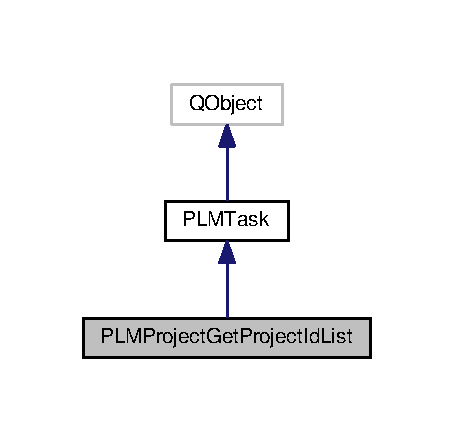
\includegraphics[width=218pt]{class_p_l_m_project_get_project_id_list__inherit__graph}
\end{center}
\end{figure}


Collaboration diagram for P\+L\+M\+Project\+Get\+Project\+Id\+List\+:\nopagebreak
\begin{figure}[H]
\begin{center}
\leavevmode
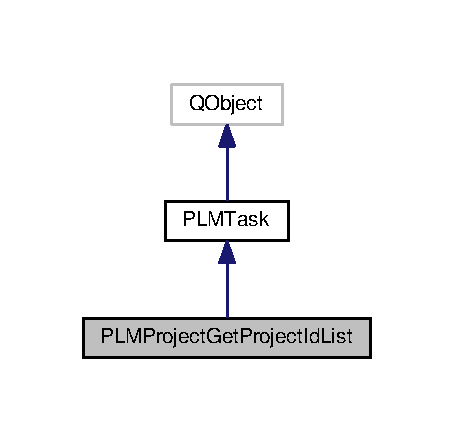
\includegraphics[width=218pt]{class_p_l_m_project_get_project_id_list__coll__graph}
\end{center}
\end{figure}
\subsection*{Public Member Functions}
\begin{DoxyCompactItemize}
\item 
void {\bfseries do\+Task} (bool $\ast$ok)\hypertarget{class_p_l_m_project_get_project_id_list_a50b4ea353012444d28099b54858f9cdb}{}\label{class_p_l_m_project_get_project_id_list_a50b4ea353012444d28099b54858f9cdb}

\end{DoxyCompactItemize}
\subsection*{Additional Inherited Members}


The documentation for this class was generated from the following file\+:\begin{DoxyCompactItemize}
\item 
src/tasks/plmprojectgetprojectidlist.\+h\end{DoxyCompactItemize}

\hypertarget{class_p_l_m_project_hub}{}\section{P\+L\+M\+Project\+Hub Class Reference}
\label{class_p_l_m_project_hub}\index{P\+L\+M\+Project\+Hub@{P\+L\+M\+Project\+Hub}}


Inheritance diagram for P\+L\+M\+Project\+Hub\+:\nopagebreak
\begin{figure}[H]
\begin{center}
\leavevmode
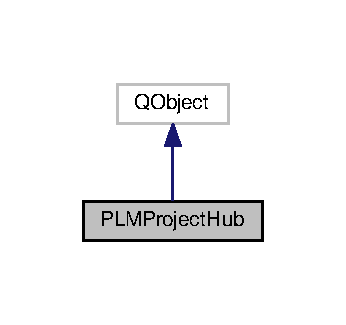
\includegraphics[width=166pt]{class_p_l_m_project_hub__inherit__graph}
\end{center}
\end{figure}


Collaboration diagram for P\+L\+M\+Project\+Hub\+:\nopagebreak
\begin{figure}[H]
\begin{center}
\leavevmode
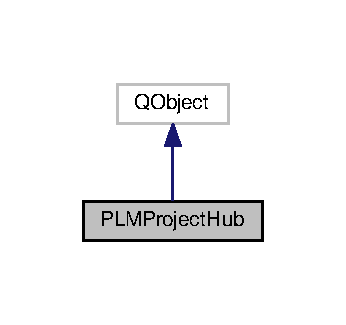
\includegraphics[width=166pt]{class_p_l_m_project_hub__coll__graph}
\end{center}
\end{figure}
\subsection*{Signals}
\begin{DoxyCompactItemize}
\item 
void {\bfseries project\+Loaded} (int project\+Id)\hypertarget{class_p_l_m_project_hub_a86ecd1dcdf8b27ca9ccd54285024406f}{}\label{class_p_l_m_project_hub_a86ecd1dcdf8b27ca9ccd54285024406f}

\item 
void {\bfseries project\+Closed} (int project\+Id)\hypertarget{class_p_l_m_project_hub_ab9bc05ad5de40a210db6f784c7ac96b0}{}\label{class_p_l_m_project_hub_ab9bc05ad5de40a210db6f784c7ac96b0}

\item 
void {\bfseries all\+Projects\+Closed} ()\hypertarget{class_p_l_m_project_hub_aec818fb471b7a5896121ab4851a166ab}{}\label{class_p_l_m_project_hub_aec818fb471b7a5896121ab4851a166ab}

\end{DoxyCompactItemize}
\subsection*{Public Member Functions}
\begin{DoxyCompactItemize}
\item 
{\bfseries P\+L\+M\+Project\+Hub} (Q\+Object $\ast$parent)\hypertarget{class_p_l_m_project_hub_a84d9d88e629f3a2a7900c2492186449f}{}\label{class_p_l_m_project_hub_a84d9d88e629f3a2a7900c2492186449f}

\item 
void {\bfseries set\+Task\+Manager} (\hyperlink{class_p_l_m_task_manager}{P\+L\+M\+Task\+Manager} $\ast$task\+Manager)\hypertarget{class_p_l_m_project_hub_a91871cb37dd5c4896dc29dd7e947f1a8}{}\label{class_p_l_m_project_hub_a91871cb37dd5c4896dc29dd7e947f1a8}

\item 
void {\bfseries load\+Project} (const Q\+String \&path)\hypertarget{class_p_l_m_project_hub_a764febea4e382622369c183730f6ab04}{}\label{class_p_l_m_project_hub_a764febea4e382622369c183730f6ab04}

\item 
void {\bfseries close\+Project} (int project\+Id)\hypertarget{class_p_l_m_project_hub_acdd01d39a52b87ed4d0a9f1ceb9fd4b9}{}\label{class_p_l_m_project_hub_acdd01d39a52b87ed4d0a9f1ceb9fd4b9}

\item 
void {\bfseries close\+All\+Projects} ()\hypertarget{class_p_l_m_project_hub_a90fa208e20446eccd2d4121fa47226c1}{}\label{class_p_l_m_project_hub_a90fa208e20446eccd2d4121fa47226c1}

\item 
Q\+List$<$ int $>$ {\bfseries get\+Project\+Id\+List} ()\hypertarget{class_p_l_m_project_hub_a7560e5168748c76ddc364c40f105f878}{}\label{class_p_l_m_project_hub_a7560e5168748c76ddc364c40f105f878}

\end{DoxyCompactItemize}


The documentation for this class was generated from the following files\+:\begin{DoxyCompactItemize}
\item 
src/plmprojecthub.\+h\item 
src/plmprojecthub.\+cpp\end{DoxyCompactItemize}

\hypertarget{class_p_l_m_project_load_project}{}\section{P\+L\+M\+Project\+Load\+Project Class Reference}
\label{class_p_l_m_project_load_project}\index{P\+L\+M\+Project\+Load\+Project@{P\+L\+M\+Project\+Load\+Project}}


Inheritance diagram for P\+L\+M\+Project\+Load\+Project\+:\nopagebreak
\begin{figure}[H]
\begin{center}
\leavevmode
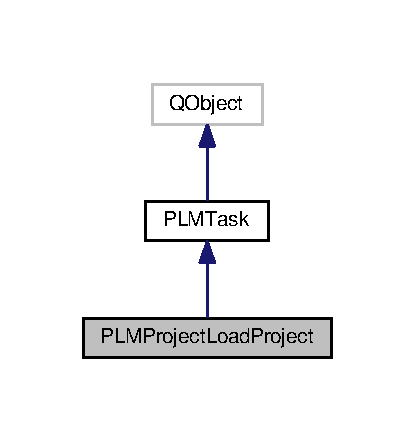
\includegraphics[width=199pt]{class_p_l_m_project_load_project__inherit__graph}
\end{center}
\end{figure}


Collaboration diagram for P\+L\+M\+Project\+Load\+Project\+:\nopagebreak
\begin{figure}[H]
\begin{center}
\leavevmode
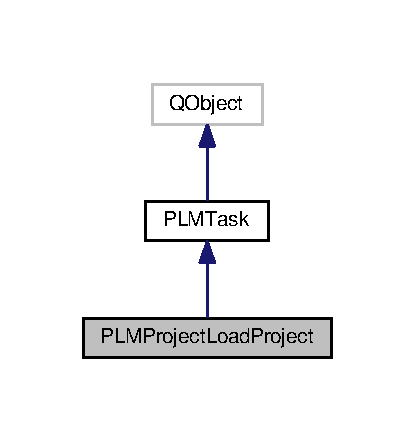
\includegraphics[width=199pt]{class_p_l_m_project_load_project__coll__graph}
\end{center}
\end{figure}
\subsection*{Public Member Functions}
\begin{DoxyCompactItemize}
\item 
{\bfseries P\+L\+M\+Project\+Load\+Project} (const Q\+String \&path)\hypertarget{class_p_l_m_project_load_project_ad84ee1f8418344d840b9cf1cce88eb0e}{}\label{class_p_l_m_project_load_project_ad84ee1f8418344d840b9cf1cce88eb0e}

\item 
void {\bfseries do\+Task} (bool $\ast$ok)\hypertarget{class_p_l_m_project_load_project_a73468241fa65d5b37ed770aeacf41ada}{}\label{class_p_l_m_project_load_project_a73468241fa65d5b37ed770aeacf41ada}

\end{DoxyCompactItemize}
\subsection*{Additional Inherited Members}


The documentation for this class was generated from the following file\+:\begin{DoxyCompactItemize}
\item 
src/tasks/plmprojectloadproject.\+h\end{DoxyCompactItemize}

\hypertarget{class_p_l_m_project_manager}{}\section{P\+L\+M\+Project\+Manager Class Reference}
\label{class_p_l_m_project_manager}\index{P\+L\+M\+Project\+Manager@{P\+L\+M\+Project\+Manager}}


Inheritance diagram for P\+L\+M\+Project\+Manager\+:\nopagebreak
\begin{figure}[H]
\begin{center}
\leavevmode
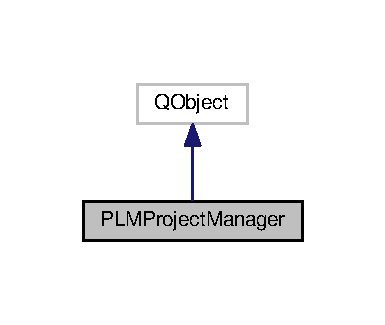
\includegraphics[width=185pt]{class_p_l_m_project_manager__inherit__graph}
\end{center}
\end{figure}


Collaboration diagram for P\+L\+M\+Project\+Manager\+:\nopagebreak
\begin{figure}[H]
\begin{center}
\leavevmode
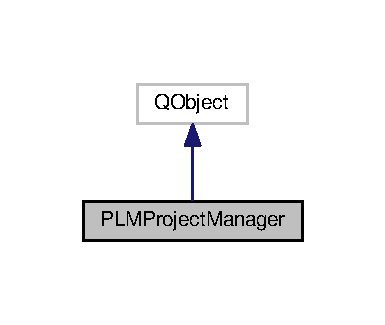
\includegraphics[width=185pt]{class_p_l_m_project_manager__coll__graph}
\end{center}
\end{figure}
\subsection*{Public Member Functions}
\begin{DoxyCompactItemize}
\item 
{\bfseries P\+L\+M\+Project\+Manager} (Q\+Object $\ast$parent)\hypertarget{class_p_l_m_project_manager_a6a2fbe712e30e3824c09de4dad21046c}{}\label{class_p_l_m_project_manager_a6a2fbe712e30e3824c09de4dad21046c}

\item 
int {\bfseries create\+New\+Empty\+Database} ()\hypertarget{class_p_l_m_project_manager_adbd9c5f0c8e884b7c42931f78940aed8}{}\label{class_p_l_m_project_manager_adbd9c5f0c8e884b7c42931f78940aed8}

\item 
int {\bfseries load\+Project} (const Q\+String \&file\+Name)\hypertarget{class_p_l_m_project_manager_a806ac2c6f430e80b3dc7c09e08eb1cf2}{}\label{class_p_l_m_project_manager_a806ac2c6f430e80b3dc7c09e08eb1cf2}

\item 
bool {\bfseries save\+Project} (int project\+Id, const Q\+String \&file\+Name)\hypertarget{class_p_l_m_project_manager_ac9d3c33f2d0af139948b88899388e029}{}\label{class_p_l_m_project_manager_ac9d3c33f2d0af139948b88899388e029}

\item 
\hyperlink{class_p_l_m_project}{P\+L\+M\+Project} $\ast$ {\bfseries project} (int project\+Id)\hypertarget{class_p_l_m_project_manager_a74d05776c72ca6964552811dcabecd02}{}\label{class_p_l_m_project_manager_a74d05776c72ca6964552811dcabecd02}

\item 
Q\+List$<$ int $>$ {\bfseries project\+Id\+List} ()\hypertarget{class_p_l_m_project_manager_a9d06c5f9870e9e866af5d5e8c91a4172}{}\label{class_p_l_m_project_manager_a9d06c5f9870e9e866af5d5e8c91a4172}

\item 
bool {\bfseries close\+Project} (int project\+Id)\hypertarget{class_p_l_m_project_manager_aec3e4e13f3effef81f52b9b2ffc91186}{}\label{class_p_l_m_project_manager_aec3e4e13f3effef81f52b9b2ffc91186}

\end{DoxyCompactItemize}
\subsection*{Static Public Member Functions}
\begin{DoxyCompactItemize}
\item 
static \hyperlink{class_p_l_m_project_manager}{P\+L\+M\+Project\+Manager} $\ast$ {\bfseries instance} ()\hypertarget{class_p_l_m_project_manager_abdea0c6b66f64d77e961d6cfbbb70a5a}{}\label{class_p_l_m_project_manager_abdea0c6b66f64d77e961d6cfbbb70a5a}

\end{DoxyCompactItemize}


The documentation for this class was generated from the following files\+:\begin{DoxyCompactItemize}
\item 
src/tasks/plmprojectmanager.\+h\item 
src/tasks/plmprojectmanager.\+cpp\end{DoxyCompactItemize}

\hypertarget{class_p_l_m_property}{}\section{P\+L\+M\+Property Class Reference}
\label{class_p_l_m_property}\index{P\+L\+M\+Property@{P\+L\+M\+Property}}


Inheritance diagram for P\+L\+M\+Property\+:\nopagebreak
\begin{figure}[H]
\begin{center}
\leavevmode
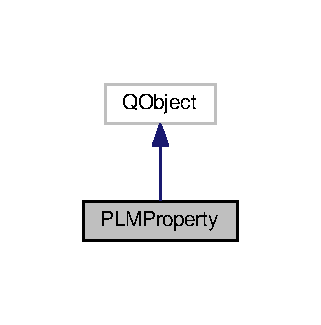
\includegraphics[width=154pt]{class_p_l_m_property__inherit__graph}
\end{center}
\end{figure}


Collaboration diagram for P\+L\+M\+Property\+:\nopagebreak
\begin{figure}[H]
\begin{center}
\leavevmode
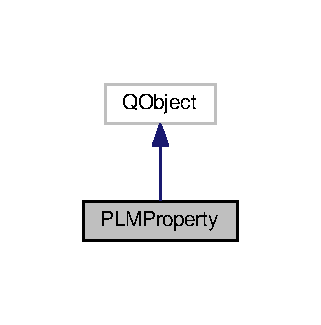
\includegraphics[width=154pt]{class_p_l_m_property__coll__graph}
\end{center}
\end{figure}
\subsection*{Public Member Functions}
\begin{DoxyCompactItemize}
\item 
{\bfseries P\+L\+M\+Property} (Q\+Object $\ast$parent, const Q\+String \&table\+Name, const Q\+String \&code\+Name, Q\+Sql\+Database sql\+Db)\hypertarget{class_p_l_m_property_a6a26fedc8e762f960d07dced138c399a}{}\label{class_p_l_m_property_a6a26fedc8e762f960d07dced138c399a}

\item 
Q\+List$<$ Q\+Hash$<$ Q\+String, Q\+Variant $>$ $>$ {\bfseries get\+All} ()\hypertarget{class_p_l_m_property_a63834de001ab1da3ed626e016524cbe3}{}\label{class_p_l_m_property_a63834de001ab1da3ed626e016524cbe3}

\item 
Q\+String\+List {\bfseries get\+All\+Headers} ()\hypertarget{class_p_l_m_property_a079eaa5c5552cd589967f5bad2a0788d}{}\label{class_p_l_m_property_a079eaa5c5552cd589967f5bad2a0788d}

\end{DoxyCompactItemize}


The documentation for this class was generated from the following files\+:\begin{DoxyCompactItemize}
\item 
src/tasks/sql/plmproperty.\+h\item 
src/tasks/sql/plmproperty.\+cpp\end{DoxyCompactItemize}

\hypertarget{class_p_l_m_sheet_tree}{}\section{P\+L\+M\+Sheet\+Tree Class Reference}
\label{class_p_l_m_sheet_tree}\index{P\+L\+M\+Sheet\+Tree@{P\+L\+M\+Sheet\+Tree}}


Inheritance diagram for P\+L\+M\+Sheet\+Tree\+:\nopagebreak
\begin{figure}[H]
\begin{center}
\leavevmode
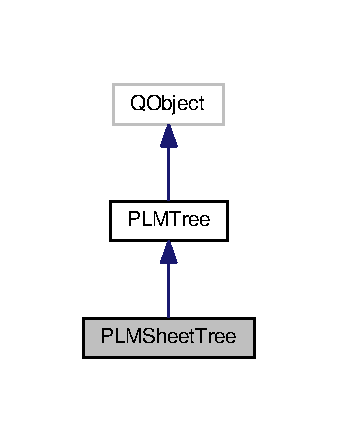
\includegraphics[width=162pt]{class_p_l_m_sheet_tree__inherit__graph}
\end{center}
\end{figure}


Collaboration diagram for P\+L\+M\+Sheet\+Tree\+:\nopagebreak
\begin{figure}[H]
\begin{center}
\leavevmode
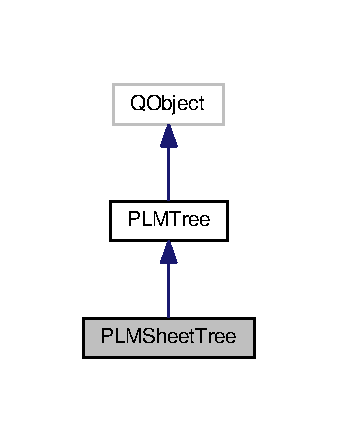
\includegraphics[width=162pt]{class_p_l_m_sheet_tree__coll__graph}
\end{center}
\end{figure}
\subsection*{Public Member Functions}
\begin{DoxyCompactItemize}
\item 
{\bfseries P\+L\+M\+Sheet\+Tree} (Q\+Object $\ast$parent, const Q\+String \&table\+Name, const Q\+String \&code\+Name, Q\+Sql\+Database sql\+Db)\hypertarget{class_p_l_m_sheet_tree_a02533e0502f7fd1bc72bcc3ef536ab5b}{}\label{class_p_l_m_sheet_tree_a02533e0502f7fd1bc72bcc3ef536ab5b}

\item 
int {\bfseries get\+Word\+Count} (int paper\+Id) const \hypertarget{class_p_l_m_sheet_tree_aab39b4df45f6b071e76ed1ddfa4b0637}{}\label{class_p_l_m_sheet_tree_aab39b4df45f6b071e76ed1ddfa4b0637}

\item 
void {\bfseries set\+Word\+Count} (int paper\+Id, int count)\hypertarget{class_p_l_m_sheet_tree_afbc394cb6beb9de2e836042c25f1e30a}{}\label{class_p_l_m_sheet_tree_afbc394cb6beb9de2e836042c25f1e30a}

\item 
int {\bfseries get\+Char\+Count} (int paper\+Id) const \hypertarget{class_p_l_m_sheet_tree_a8458181a36e69f8c0275141de15a058f}{}\label{class_p_l_m_sheet_tree_a8458181a36e69f8c0275141de15a058f}

\item 
void {\bfseries set\+Char\+Count} (int paper\+Id, int count)\hypertarget{class_p_l_m_sheet_tree_a2cc0cfe04bae86453675b3aeadea3581}{}\label{class_p_l_m_sheet_tree_a2cc0cfe04bae86453675b3aeadea3581}

\end{DoxyCompactItemize}
\subsection*{Additional Inherited Members}


The documentation for this class was generated from the following files\+:\begin{DoxyCompactItemize}
\item 
src/tasks/sql/tree/plmsheettree.\+h\item 
src/tasks/sql/tree/plmsheettree.\+cpp\end{DoxyCompactItemize}

\hypertarget{class_p_l_m_signal_hub}{}\section{P\+L\+M\+Signal\+Hub Class Reference}
\label{class_p_l_m_signal_hub}\index{P\+L\+M\+Signal\+Hub@{P\+L\+M\+Signal\+Hub}}


Inheritance diagram for P\+L\+M\+Signal\+Hub\+:\nopagebreak
\begin{figure}[H]
\begin{center}
\leavevmode
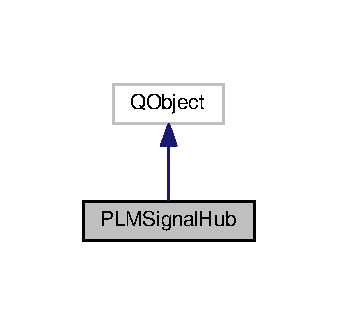
\includegraphics[width=162pt]{class_p_l_m_signal_hub__inherit__graph}
\end{center}
\end{figure}


Collaboration diagram for P\+L\+M\+Signal\+Hub\+:\nopagebreak
\begin{figure}[H]
\begin{center}
\leavevmode
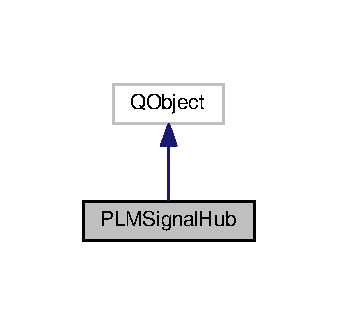
\includegraphics[width=162pt]{class_p_l_m_signal_hub__coll__graph}
\end{center}
\end{figure}
\subsection*{Public Member Functions}
\begin{DoxyCompactItemize}
\item 
{\bfseries P\+L\+M\+Signal\+Hub} (Q\+Object $\ast$parent)\hypertarget{class_p_l_m_signal_hub_adafe7723e20aa1621654cb59b42591a9}{}\label{class_p_l_m_signal_hub_adafe7723e20aa1621654cb59b42591a9}

\end{DoxyCompactItemize}


The documentation for this class was generated from the following file\+:\begin{DoxyCompactItemize}
\item 
src/plmsignalhub.\+h\end{DoxyCompactItemize}

\hypertarget{class_p_l_m_task}{}\section{P\+L\+M\+Task Class Reference}
\label{class_p_l_m_task}\index{P\+L\+M\+Task@{P\+L\+M\+Task}}


Inheritance diagram for P\+L\+M\+Task\+:\nopagebreak
\begin{figure}[H]
\begin{center}
\leavevmode
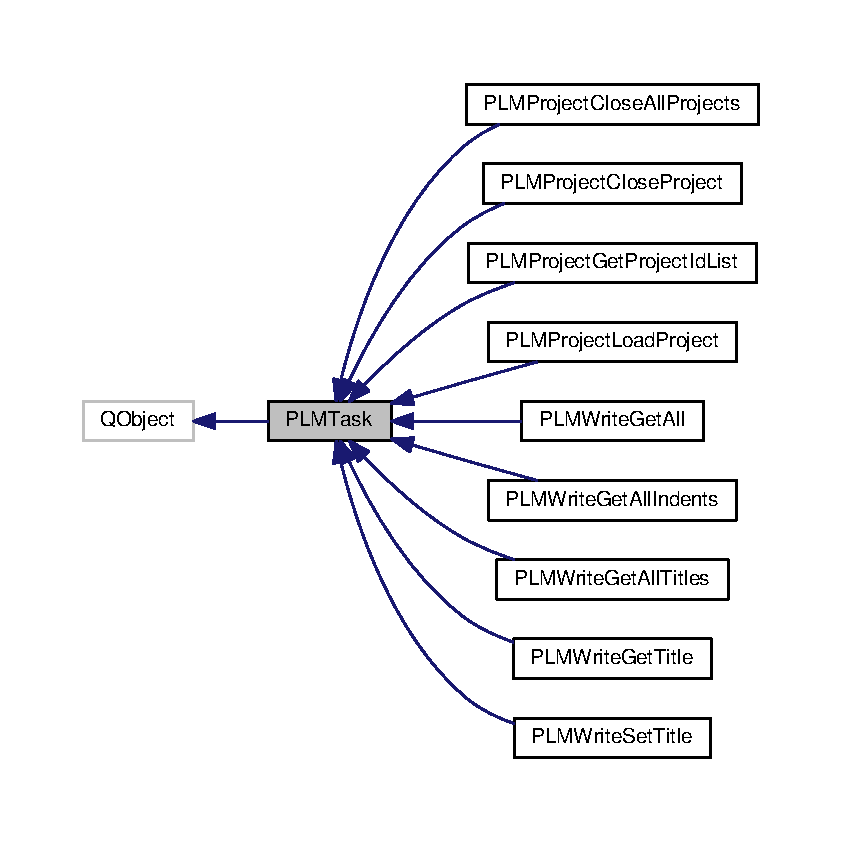
\includegraphics[width=350pt]{class_p_l_m_task__inherit__graph}
\end{center}
\end{figure}


Collaboration diagram for P\+L\+M\+Task\+:\nopagebreak
\begin{figure}[H]
\begin{center}
\leavevmode
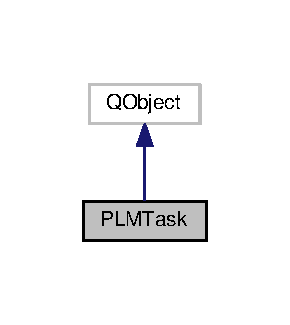
\includegraphics[width=139pt]{class_p_l_m_task__coll__graph}
\end{center}
\end{figure}
\subsection*{Public Types}
\begin{DoxyCompactItemize}
\item 
enum {\bfseries Type} \{ {\bfseries Getter}, 
{\bfseries Setter}
 \}\hypertarget{class_p_l_m_task_a9e0f58ff71fe4908bf42d3b9275df359}{}\label{class_p_l_m_task_a9e0f58ff71fe4908bf42d3b9275df359}

\end{DoxyCompactItemize}
\subsection*{Signals}
\begin{DoxyCompactItemize}
\item 
void {\bfseries task\+Finished} ()\hypertarget{class_p_l_m_task_a42d0acbdca59ddb213499193d80d9dcb}{}\label{class_p_l_m_task_a42d0acbdca59ddb213499193d80d9dcb}

\item 
void {\bfseries task\+Started} ()\hypertarget{class_p_l_m_task_a3e4ffc2ec649612a18676de0d3b90cca}{}\label{class_p_l_m_task_a3e4ffc2ec649612a18676de0d3b90cca}

\item 
void {\bfseries error\+Sent} (const Q\+String \&error)\hypertarget{class_p_l_m_task_a6838dfdac49090cffeb26591dc29736d}{}\label{class_p_l_m_task_a6838dfdac49090cffeb26591dc29736d}

\end{DoxyCompactItemize}
\subsection*{Public Member Functions}
\begin{DoxyCompactItemize}
\item 
virtual void {\bfseries do\+Task} (bool $\ast$ok)=0\hypertarget{class_p_l_m_task_a3daa83d5290573d976b49bf41e969b72}{}\label{class_p_l_m_task_a3daa83d5290573d976b49bf41e969b72}

\item 
Type {\bfseries type} () const \hypertarget{class_p_l_m_task_adbcf19c6cd19a384154f0e57617d23b1}{}\label{class_p_l_m_task_adbcf19c6cd19a384154f0e57617d23b1}

\item 
Q\+Variant {\bfseries return\+Value} () const \hypertarget{class_p_l_m_task_a50be638d1d32a8ccf738e65c1d49f022}{}\label{class_p_l_m_task_a50be638d1d32a8ccf738e65c1d49f022}

\item 
Q\+List$<$ Q\+Hash$<$ Q\+String, Q\+Variant $>$ $>$ {\bfseries return\+Value\+Get\+All} () const \hypertarget{class_p_l_m_task_aa0421360e3640a07e4aa5a194082078f}{}\label{class_p_l_m_task_aa0421360e3640a07e4aa5a194082078f}

\item 
Q\+Hash$<$ int, Q\+Variant $>$ {\bfseries return\+Value\+Hash} () const \hypertarget{class_p_l_m_task_a99059e1a7ff7d2206f5a561fb05fbdd6}{}\label{class_p_l_m_task_a99059e1a7ff7d2206f5a561fb05fbdd6}

\item 
Q\+List$<$ Q\+Variant $>$ {\bfseries return\+Value\+List} () const \hypertarget{class_p_l_m_task_a58e455cbe80db6fdc6c4a2d920a342ff}{}\label{class_p_l_m_task_a58e455cbe80db6fdc6c4a2d920a342ff}

\item 
void {\bfseries set\+Return\+Value} (const Q\+Variant \&return\+Value)\hypertarget{class_p_l_m_task_a974b3db04ac20afc1a0dda65cd3afe1b}{}\label{class_p_l_m_task_a974b3db04ac20afc1a0dda65cd3afe1b}

\item 
void {\bfseries set\+Return\+Value\+Get\+All} (const Q\+List$<$ Q\+Hash$<$ Q\+String, Q\+Variant $>$ $>$ \&return\+Value)\hypertarget{class_p_l_m_task_ad4cdd4defb5b93c85360e2451837bd17}{}\label{class_p_l_m_task_ad4cdd4defb5b93c85360e2451837bd17}

\item 
void {\bfseries set\+Return\+Value\+Hash} (const Q\+Hash$<$ int, Q\+Variant $>$ \&return\+Value)\hypertarget{class_p_l_m_task_a8b0bca01fb1918f255d7a7a03aed5966}{}\label{class_p_l_m_task_a8b0bca01fb1918f255d7a7a03aed5966}

\item 
void {\bfseries set\+Return\+Value\+List} (const Q\+List$<$ Q\+Variant $>$ \&return\+Value)\hypertarget{class_p_l_m_task_a021bd4af36bcbffbf8673747b4ab22fe}{}\label{class_p_l_m_task_a021bd4af36bcbffbf8673747b4ab22fe}

\end{DoxyCompactItemize}
\subsection*{Protected Member Functions}
\begin{DoxyCompactItemize}
\item 
void {\bfseries set\+Type} (const Type \&\+\_\+type)\hypertarget{class_p_l_m_task_a51fa5c4fd2dbffc2df4506b55107b0a7}{}\label{class_p_l_m_task_a51fa5c4fd2dbffc2df4506b55107b0a7}

\end{DoxyCompactItemize}


The documentation for this class was generated from the following file\+:\begin{DoxyCompactItemize}
\item 
src/tasks/plmtask.\+h\end{DoxyCompactItemize}

\hypertarget{class_p_l_m_task_bridge}{}\section{P\+L\+M\+Task\+Bridge Class Reference}
\label{class_p_l_m_task_bridge}\index{P\+L\+M\+Task\+Bridge@{P\+L\+M\+Task\+Bridge}}


Inheritance diagram for P\+L\+M\+Task\+Bridge\+:\nopagebreak
\begin{figure}[H]
\begin{center}
\leavevmode
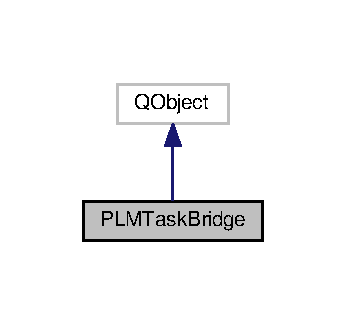
\includegraphics[width=166pt]{class_p_l_m_task_bridge__inherit__graph}
\end{center}
\end{figure}


Collaboration diagram for P\+L\+M\+Task\+Bridge\+:\nopagebreak
\begin{figure}[H]
\begin{center}
\leavevmode
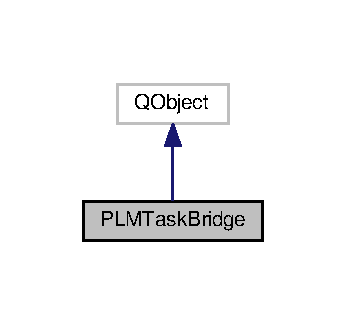
\includegraphics[width=166pt]{class_p_l_m_task_bridge__coll__graph}
\end{center}
\end{figure}
\subsection*{Public Slots}
\begin{DoxyCompactItemize}
\item 
void {\bfseries append\+Task} (\hyperlink{class_p_l_m_task}{P\+L\+M\+Task} $\ast$task)\hypertarget{class_p_l_m_task_bridge_af4a7b8e57da51a1bcd691844599ae3ac}{}\label{class_p_l_m_task_bridge_af4a7b8e57da51a1bcd691844599ae3ac}

\item 
void {\bfseries send\+Return\+Value} ()\hypertarget{class_p_l_m_task_bridge_ab48afaf8e7a8ef318623be1da97b2981}{}\label{class_p_l_m_task_bridge_ab48afaf8e7a8ef318623be1da97b2981}

\end{DoxyCompactItemize}
\subsection*{Signals}
\begin{DoxyCompactItemize}
\item 
void {\bfseries return\+Value\+Sent} (const Q\+Variant \&value)\hypertarget{class_p_l_m_task_bridge_ad144c31db4e0f5d23092eab900a7298f}{}\label{class_p_l_m_task_bridge_ad144c31db4e0f5d23092eab900a7298f}

\item 
void {\bfseries return\+Value\+Sent\+Get\+All} (const Q\+List$<$ Q\+Hash$<$ Q\+String, Q\+Variant $>$ $>$ \&value)\hypertarget{class_p_l_m_task_bridge_ae8267e49794081614601e24b9eca0144}{}\label{class_p_l_m_task_bridge_ae8267e49794081614601e24b9eca0144}

\item 
void {\bfseries return\+Value\+Sent\+Hash} (const Q\+Hash$<$ int, Q\+Variant $>$ \&value)\hypertarget{class_p_l_m_task_bridge_a5e4267de935444128677563c0aa91798}{}\label{class_p_l_m_task_bridge_a5e4267de935444128677563c0aa91798}

\item 
void {\bfseries return\+Value\+Sent\+List} (const Q\+List$<$ Q\+Variant $>$ \&value)\hypertarget{class_p_l_m_task_bridge_a4dff354383d5541cdb4bb50e96eeb32c}{}\label{class_p_l_m_task_bridge_a4dff354383d5541cdb4bb50e96eeb32c}

\item 
void {\bfseries error\+Sent} ()\hypertarget{class_p_l_m_task_bridge_a112c2296d8833638e8c4e67f3c97a494}{}\label{class_p_l_m_task_bridge_a112c2296d8833638e8c4e67f3c97a494}

\item 
void {\bfseries stop\+Loop\+Event} ()\hypertarget{class_p_l_m_task_bridge_ab0d85fbde08b2646e221253fc303360a}{}\label{class_p_l_m_task_bridge_ab0d85fbde08b2646e221253fc303360a}

\end{DoxyCompactItemize}


The documentation for this class was generated from the following files\+:\begin{DoxyCompactItemize}
\item 
src/tasks/plmtaskbridge.\+h\item 
src/tasks/plmtaskbridge.\+cpp\end{DoxyCompactItemize}

\hypertarget{class_p_l_m_task_error}{}\section{P\+L\+M\+Task\+Error Class Reference}
\label{class_p_l_m_task_error}\index{P\+L\+M\+Task\+Error@{P\+L\+M\+Task\+Error}}


Inheritance diagram for P\+L\+M\+Task\+Error\+:\nopagebreak
\begin{figure}[H]
\begin{center}
\leavevmode
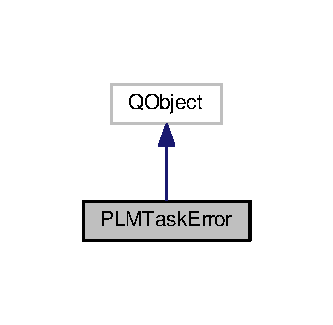
\includegraphics[width=160pt]{class_p_l_m_task_error__inherit__graph}
\end{center}
\end{figure}


Collaboration diagram for P\+L\+M\+Task\+Error\+:\nopagebreak
\begin{figure}[H]
\begin{center}
\leavevmode
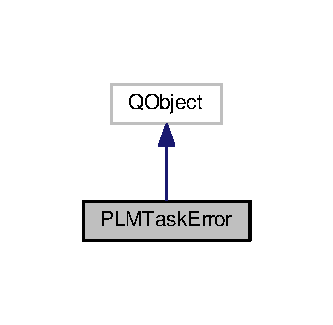
\includegraphics[width=160pt]{class_p_l_m_task_error__coll__graph}
\end{center}
\end{figure}
\subsection*{Signals}
\begin{DoxyCompactItemize}
\item 
void {\bfseries error\+Sent} (const Q\+String \&error\+Code, const Q\+String \&origin, const Q\+String \&message)\hypertarget{class_p_l_m_task_error_a802e611c3c002e3f113d852e02ac572f}{}\label{class_p_l_m_task_error_a802e611c3c002e3f113d852e02ac572f}

\end{DoxyCompactItemize}
\subsection*{Public Member Functions}
\begin{DoxyCompactItemize}
\item 
{\bfseries P\+L\+M\+Task\+Error} (Q\+Object $\ast$parent)\hypertarget{class_p_l_m_task_error_a4fd8fe77d074d6f8fa5d1595442d5a79}{}\label{class_p_l_m_task_error_a4fd8fe77d074d6f8fa5d1595442d5a79}

\end{DoxyCompactItemize}
\subsection*{Static Public Member Functions}
\begin{DoxyCompactItemize}
\item 
static \hyperlink{class_p_l_m_task_error}{P\+L\+M\+Task\+Error} $\ast$ {\bfseries instance} ()\hypertarget{class_p_l_m_task_error_a9e4a0fa94c692b736c2a31be19f413ba}{}\label{class_p_l_m_task_error_a9e4a0fa94c692b736c2a31be19f413ba}

\end{DoxyCompactItemize}


The documentation for this class was generated from the following files\+:\begin{DoxyCompactItemize}
\item 
src/tasks/plmtaskerror.\+h\item 
src/tasks/plmtaskerror.\+cpp\end{DoxyCompactItemize}

\hypertarget{class_p_l_m_task_manager}{}\section{P\+L\+M\+Task\+Manager Class Reference}
\label{class_p_l_m_task_manager}\index{P\+L\+M\+Task\+Manager@{P\+L\+M\+Task\+Manager}}


Inheritance diagram for P\+L\+M\+Task\+Manager\+:\nopagebreak
\begin{figure}[H]
\begin{center}
\leavevmode
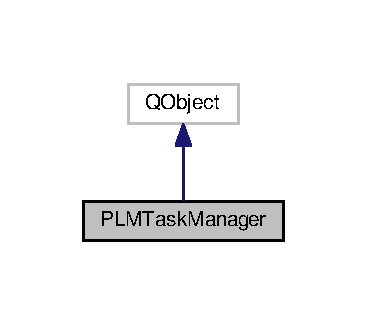
\includegraphics[width=176pt]{class_p_l_m_task_manager__inherit__graph}
\end{center}
\end{figure}


Collaboration diagram for P\+L\+M\+Task\+Manager\+:\nopagebreak
\begin{figure}[H]
\begin{center}
\leavevmode
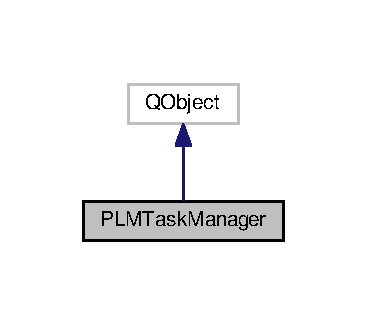
\includegraphics[width=176pt]{class_p_l_m_task_manager__coll__graph}
\end{center}
\end{figure}
\subsection*{Signals}
\begin{DoxyCompactItemize}
\item 
void {\bfseries append\+Task\+Sent} (\hyperlink{class_p_l_m_task}{P\+L\+M\+Task} $\ast$task)\hypertarget{class_p_l_m_task_manager_a96f657566aca5d6647ff5d417e216014}{}\label{class_p_l_m_task_manager_a96f657566aca5d6647ff5d417e216014}

\item 
void {\bfseries return\+Value\+Asked} ()\hypertarget{class_p_l_m_task_manager_ab99b42a981d16d1fddd24e36aaa50c6b}{}\label{class_p_l_m_task_manager_ab99b42a981d16d1fddd24e36aaa50c6b}

\end{DoxyCompactItemize}
\subsection*{Public Member Functions}
\begin{DoxyCompactItemize}
\item 
\hyperlink{class_p_l_m_task_manager_adc747855b455e6ee1ff2a4499e374084}{P\+L\+M\+Task\+Manager} (Q\+Object $\ast$parent=0)
\begin{DoxyCompactList}\small\item\em \hyperlink{class_p_l_m_task_manager_adc747855b455e6ee1ff2a4499e374084}{P\+L\+M\+Task\+Manager\+::\+P\+L\+M\+Task\+Manager}. \end{DoxyCompactList}\item 
void {\bfseries append} (\hyperlink{class_p_l_m_task}{P\+L\+M\+Task} $\ast$task)\hypertarget{class_p_l_m_task_manager_ac325aaabace9d6432f12ac31207417b9}{}\label{class_p_l_m_task_manager_ac325aaabace9d6432f12ac31207417b9}

\item 
Q\+Variant {\bfseries return\+Value} ()\hypertarget{class_p_l_m_task_manager_a2831c52e4fd53cdaaad72720f745738e}{}\label{class_p_l_m_task_manager_a2831c52e4fd53cdaaad72720f745738e}

\item 
Q\+List$<$ Q\+Hash$<$ Q\+String, Q\+Variant $>$ $>$ {\bfseries return\+Value\+Get\+All} ()\hypertarget{class_p_l_m_task_manager_a5f9c80e38e7514adc24821e5f18d46c9}{}\label{class_p_l_m_task_manager_a5f9c80e38e7514adc24821e5f18d46c9}

\item 
Q\+Hash$<$ int, Q\+Variant $>$ {\bfseries return\+Value\+Hash} ()\hypertarget{class_p_l_m_task_manager_a730294c4fc26e088b90428b238696a1c}{}\label{class_p_l_m_task_manager_a730294c4fc26e088b90428b238696a1c}

\item 
Q\+List$<$ Q\+Variant $>$ {\bfseries return\+Value\+List} ()\hypertarget{class_p_l_m_task_manager_af891396f186d27d26bd07472e24f958c}{}\label{class_p_l_m_task_manager_af891396f186d27d26bd07472e24f958c}

\end{DoxyCompactItemize}


\subsection{Constructor \& Destructor Documentation}
\index{P\+L\+M\+Task\+Manager@{P\+L\+M\+Task\+Manager}!P\+L\+M\+Task\+Manager@{P\+L\+M\+Task\+Manager}}
\index{P\+L\+M\+Task\+Manager@{P\+L\+M\+Task\+Manager}!P\+L\+M\+Task\+Manager@{P\+L\+M\+Task\+Manager}}
\subsubsection[{\texorpdfstring{P\+L\+M\+Task\+Manager(\+Q\+Object $\ast$parent=0)}{PLMTaskManager(QObject *parent=0)}}]{\setlength{\rightskip}{0pt plus 5cm}P\+L\+M\+Task\+Manager\+::\+P\+L\+M\+Task\+Manager (
\begin{DoxyParamCaption}
\item[{Q\+Object $\ast$}]{parent = {\ttfamily 0}}
\end{DoxyParamCaption}
)\hspace{0.3cm}{\ttfamily [explicit]}}\hypertarget{class_p_l_m_task_manager_adc747855b455e6ee1ff2a4499e374084}{}\label{class_p_l_m_task_manager_adc747855b455e6ee1ff2a4499e374084}


\hyperlink{class_p_l_m_task_manager_adc747855b455e6ee1ff2a4499e374084}{P\+L\+M\+Task\+Manager\+::\+P\+L\+M\+Task\+Manager}. 


\begin{DoxyParams}{Parameters}
{\em parent} & \\
\hline
\end{DoxyParams}


The documentation for this class was generated from the following files\+:\begin{DoxyCompactItemize}
\item 
src/plmtaskmanager.\+h\item 
src/plmtaskmanager.\+cpp\end{DoxyCompactItemize}

\hypertarget{class_p_l_m_tree}{}\section{P\+L\+M\+Tree Class Reference}
\label{class_p_l_m_tree}\index{P\+L\+M\+Tree@{P\+L\+M\+Tree}}


Inheritance diagram for P\+L\+M\+Tree\+:\nopagebreak
\begin{figure}[H]
\begin{center}
\leavevmode
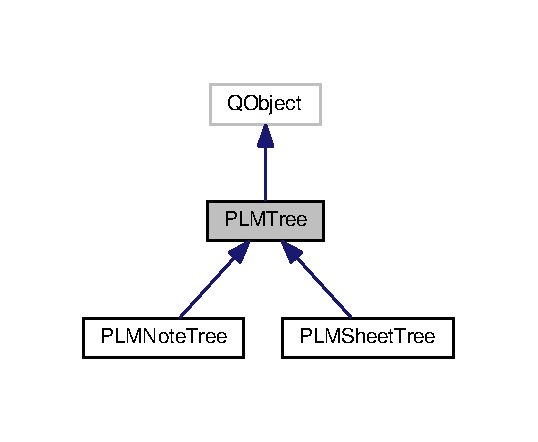
\includegraphics[width=258pt]{class_p_l_m_tree__inherit__graph}
\end{center}
\end{figure}


Collaboration diagram for P\+L\+M\+Tree\+:\nopagebreak
\begin{figure}[H]
\begin{center}
\leavevmode
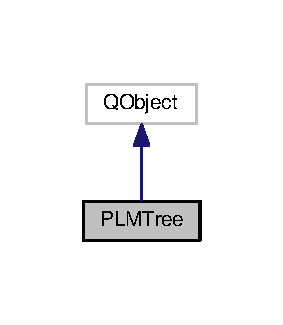
\includegraphics[width=136pt]{class_p_l_m_tree__coll__graph}
\end{center}
\end{figure}
\subsection*{Public Member Functions}
\begin{DoxyCompactItemize}
\item 
{\bfseries P\+L\+M\+Tree} (Q\+Object $\ast$parent, const Q\+String \&table\+Name, const Q\+String \&code\+Name, Q\+Sql\+Database sql\+Db)\hypertarget{class_p_l_m_tree_a27464361b0cb61431985f7f2d24fe627}{}\label{class_p_l_m_tree_a27464361b0cb61431985f7f2d24fe627}

\item 
Q\+List$<$ Q\+Hash$<$ Q\+String, Q\+Variant $>$ $>$ {\bfseries get\+All} ()\hypertarget{class_p_l_m_tree_a7d73d7331476825a8c21d6f93cb30dd7}{}\label{class_p_l_m_tree_a7d73d7331476825a8c21d6f93cb30dd7}

\item 
Q\+String\+List {\bfseries get\+All\+Headers} ()\hypertarget{class_p_l_m_tree_acc38394cc2001c3a98d364f2a8557568}{}\label{class_p_l_m_tree_acc38394cc2001c3a98d364f2a8557568}

\item 
Q\+Hash$<$ int, Q\+Variant $>$ {\bfseries get\+All\+Values} (const Q\+String \&header)\hypertarget{class_p_l_m_tree_a3d599533c1ff07ec6dfa0934eefba514}{}\label{class_p_l_m_tree_a3d599533c1ff07ec6dfa0934eefba514}

\item 
Q\+Variant {\bfseries get\+Content} (int paper\+Id) const \hypertarget{class_p_l_m_tree_a88e71f3eec07a041302f808cc86c413a}{}\label{class_p_l_m_tree_a88e71f3eec07a041302f808cc86c413a}

\item 
void {\bfseries set\+Content} (int paper\+Id, const Q\+Variant \&value)\hypertarget{class_p_l_m_tree_a806c2ed32ff05a28adf428278511b982}{}\label{class_p_l_m_tree_a806c2ed32ff05a28adf428278511b982}

\item 
Q\+String {\bfseries get\+Title} (int paper\+Id) const \hypertarget{class_p_l_m_tree_a428aabb32040c2296f172fc38b54b3cd}{}\label{class_p_l_m_tree_a428aabb32040c2296f172fc38b54b3cd}

\item 
void {\bfseries set\+Title} (int paper\+Id, const Q\+String \&value)\hypertarget{class_p_l_m_tree_a969316b62ad9871e09f1985c27af2a14}{}\label{class_p_l_m_tree_a969316b62ad9871e09f1985c27af2a14}

\item 
Q\+List$<$ int $>$ {\bfseries add\+New\+Child\+Papers} (int parent\+Id, int number)\hypertarget{class_p_l_m_tree_ae749d577145f9155fac7659a6c532940}{}\label{class_p_l_m_tree_ae749d577145f9155fac7659a6c532940}

\item 
Q\+List$<$ int $>$ {\bfseries add\+New\+Papers\+By} (int paper\+Id, int number)\hypertarget{class_p_l_m_tree_aec5b6658b0b45988ec4f69bfba1a4ac4}{}\label{class_p_l_m_tree_aec5b6658b0b45988ec4f69bfba1a4ac4}

\item 
void {\bfseries move\+Papers\+As\+Child\+Of} (Q\+List$<$ int $>$ paper\+Id\+List, int dest\+Id)\hypertarget{class_p_l_m_tree_a3a316ce33f1affda29b08da509603cc4}{}\label{class_p_l_m_tree_a3a316ce33f1affda29b08da509603cc4}

\item 
void {\bfseries move\+Papers\+Above} (Q\+List$<$ int $>$ paper\+Id\+List, int dest\+Id)\hypertarget{class_p_l_m_tree_a8779975366d60197cb164d8992fc5753}{}\label{class_p_l_m_tree_a8779975366d60197cb164d8992fc5753}

\item 
void {\bfseries move\+Papers\+Below} (Q\+List$<$ int $>$ paper\+Id\+List, int dest\+Id)\hypertarget{class_p_l_m_tree_a830691cee97b31eedf435a449825463a}{}\label{class_p_l_m_tree_a830691cee97b31eedf435a449825463a}

\end{DoxyCompactItemize}
\subsection*{Protected Member Functions}
\begin{DoxyCompactItemize}
\item 
Q\+String {\bfseries table\+Name} () const \hypertarget{class_p_l_m_tree_a4db68c2f87621e8c5c9312d50708e555}{}\label{class_p_l_m_tree_a4db68c2f87621e8c5c9312d50708e555}

\item 
Q\+String {\bfseries id\+Name} () const \hypertarget{class_p_l_m_tree_a51d5db6a6d3eaaee86c0f34dad9c937d}{}\label{class_p_l_m_tree_a51d5db6a6d3eaaee86c0f34dad9c937d}

\item 
Q\+Sql\+Database {\bfseries sql\+Db} () const \hypertarget{class_p_l_m_tree_a4f35a008994f96e0c6760f9777a39af9}{}\label{class_p_l_m_tree_a4f35a008994f96e0c6760f9777a39af9}

\item 
Q\+List$<$ int $>$ {\bfseries add\+New\+Child\+Papers} (int parent\+Id, int number, bool commit)\hypertarget{class_p_l_m_tree_a1663af74680cd9b833596f0967d2726e}{}\label{class_p_l_m_tree_a1663af74680cd9b833596f0967d2726e}

\item 
Q\+List$<$ int $>$ {\bfseries add\+New\+Papers\+By} (int paper\+Id, int number, bool commit)\hypertarget{class_p_l_m_tree_a451e4d8ca330b487405e1f0071770b82}{}\label{class_p_l_m_tree_a451e4d8ca330b487405e1f0071770b82}

\item 
void {\bfseries move\+Papers\+As\+Child\+Of} (Q\+List$<$ int $>$ paper\+Id\+List, int dest\+Id, bool commit)\hypertarget{class_p_l_m_tree_a6df2d0135fc295135c55178486e4643e}{}\label{class_p_l_m_tree_a6df2d0135fc295135c55178486e4643e}

\item 
void {\bfseries move\+Papers\+Above} (Q\+List$<$ int $>$ paper\+Id\+List, int dest\+Id, bool commit)\hypertarget{class_p_l_m_tree_a817dafc13f96873f27dbe29db3913105}{}\label{class_p_l_m_tree_a817dafc13f96873f27dbe29db3913105}

\item 
void {\bfseries move\+Papers\+Below} (Q\+List$<$ int $>$ paper\+Id\+List, int dest\+Id, bool commit)\hypertarget{class_p_l_m_tree_a39d23102d9bd34022f00fb2e55465efb}{}\label{class_p_l_m_tree_a39d23102d9bd34022f00fb2e55465efb}

\end{DoxyCompactItemize}


The documentation for this class was generated from the following files\+:\begin{DoxyCompactItemize}
\item 
src/tasks/sql/tree/plmtree.\+h\item 
src/tasks/sql/tree/plmtree.\+cpp\end{DoxyCompactItemize}

\hypertarget{class_p_l_m_write_get_all}{}\section{P\+L\+M\+Write\+Get\+All Class Reference}
\label{class_p_l_m_write_get_all}\index{P\+L\+M\+Write\+Get\+All@{P\+L\+M\+Write\+Get\+All}}


Inheritance diagram for P\+L\+M\+Write\+Get\+All\+:\nopagebreak
\begin{figure}[H]
\begin{center}
\leavevmode
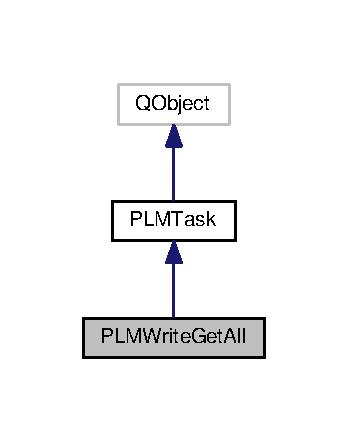
\includegraphics[width=167pt]{class_p_l_m_write_get_all__inherit__graph}
\end{center}
\end{figure}


Collaboration diagram for P\+L\+M\+Write\+Get\+All\+:\nopagebreak
\begin{figure}[H]
\begin{center}
\leavevmode
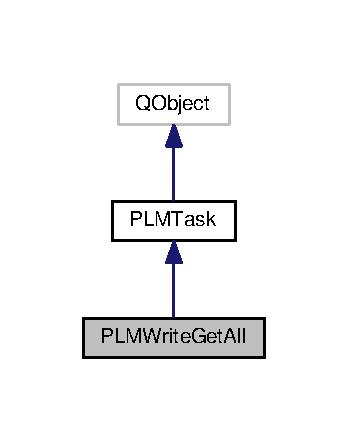
\includegraphics[width=167pt]{class_p_l_m_write_get_all__coll__graph}
\end{center}
\end{figure}
\subsection*{Public Member Functions}
\begin{DoxyCompactItemize}
\item 
{\bfseries P\+L\+M\+Write\+Get\+All} (int project\+Id)\hypertarget{class_p_l_m_write_get_all_a204d4a61ac4673ff6d51d50153be0759}{}\label{class_p_l_m_write_get_all_a204d4a61ac4673ff6d51d50153be0759}

\item 
void {\bfseries do\+Task} (bool $\ast$ok)\hypertarget{class_p_l_m_write_get_all_a20b0973f10abfdb200429e7e4a6bdbe5}{}\label{class_p_l_m_write_get_all_a20b0973f10abfdb200429e7e4a6bdbe5}

\end{DoxyCompactItemize}
\subsection*{Additional Inherited Members}


The documentation for this class was generated from the following file\+:\begin{DoxyCompactItemize}
\item 
src/tasks/plmwritegetall.\+h\end{DoxyCompactItemize}

\hypertarget{class_p_l_m_write_get_all_indents}{}\section{P\+L\+M\+Write\+Get\+All\+Indents Class Reference}
\label{class_p_l_m_write_get_all_indents}\index{P\+L\+M\+Write\+Get\+All\+Indents@{P\+L\+M\+Write\+Get\+All\+Indents}}


Inheritance diagram for P\+L\+M\+Write\+Get\+All\+Indents\+:\nopagebreak
\begin{figure}[H]
\begin{center}
\leavevmode
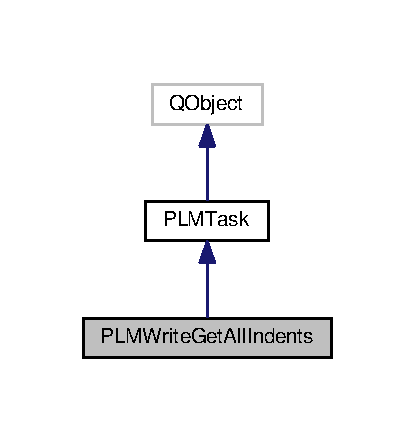
\includegraphics[width=199pt]{class_p_l_m_write_get_all_indents__inherit__graph}
\end{center}
\end{figure}


Collaboration diagram for P\+L\+M\+Write\+Get\+All\+Indents\+:\nopagebreak
\begin{figure}[H]
\begin{center}
\leavevmode
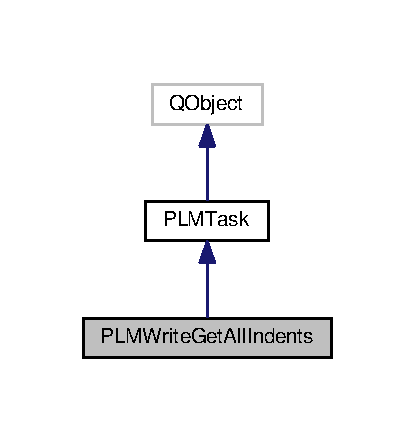
\includegraphics[width=199pt]{class_p_l_m_write_get_all_indents__coll__graph}
\end{center}
\end{figure}
\subsection*{Public Member Functions}
\begin{DoxyCompactItemize}
\item 
{\bfseries P\+L\+M\+Write\+Get\+All\+Indents} (int project\+Id)\hypertarget{class_p_l_m_write_get_all_indents_a6df034e7206f4009cb8e66456d4c878c}{}\label{class_p_l_m_write_get_all_indents_a6df034e7206f4009cb8e66456d4c878c}

\item 
void {\bfseries do\+Task} (bool $\ast$ok)\hypertarget{class_p_l_m_write_get_all_indents_a49f8c56451f23d8ffbb1b58df9c18007}{}\label{class_p_l_m_write_get_all_indents_a49f8c56451f23d8ffbb1b58df9c18007}

\end{DoxyCompactItemize}
\subsection*{Additional Inherited Members}


The documentation for this class was generated from the following file\+:\begin{DoxyCompactItemize}
\item 
src/tasks/plmwritegetallindents.\+h\end{DoxyCompactItemize}

\hypertarget{class_p_l_m_write_get_all_titles}{}\section{P\+L\+M\+Write\+Get\+All\+Titles Class Reference}
\label{class_p_l_m_write_get_all_titles}\index{P\+L\+M\+Write\+Get\+All\+Titles@{P\+L\+M\+Write\+Get\+All\+Titles}}


Inheritance diagram for P\+L\+M\+Write\+Get\+All\+Titles\+:\nopagebreak
\begin{figure}[H]
\begin{center}
\leavevmode
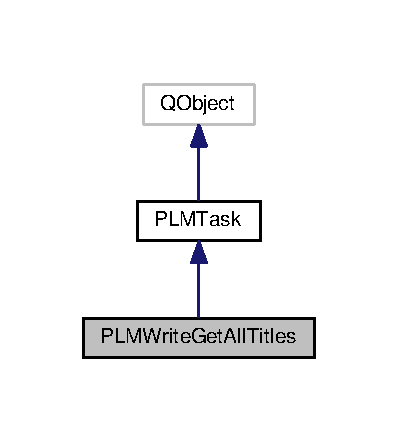
\includegraphics[width=191pt]{class_p_l_m_write_get_all_titles__inherit__graph}
\end{center}
\end{figure}


Collaboration diagram for P\+L\+M\+Write\+Get\+All\+Titles\+:\nopagebreak
\begin{figure}[H]
\begin{center}
\leavevmode
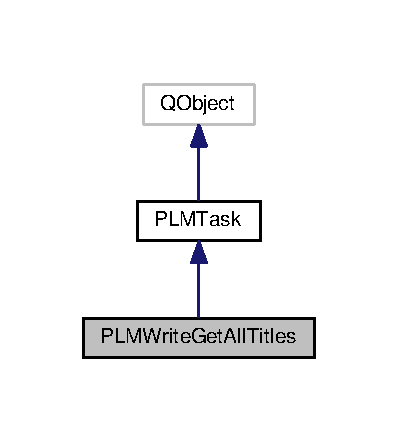
\includegraphics[width=191pt]{class_p_l_m_write_get_all_titles__coll__graph}
\end{center}
\end{figure}
\subsection*{Public Member Functions}
\begin{DoxyCompactItemize}
\item 
{\bfseries P\+L\+M\+Write\+Get\+All\+Titles} (int project\+Id)\hypertarget{class_p_l_m_write_get_all_titles_a7f18199918100a2ffa04bace3cef3449}{}\label{class_p_l_m_write_get_all_titles_a7f18199918100a2ffa04bace3cef3449}

\item 
void {\bfseries do\+Task} (bool $\ast$ok)\hypertarget{class_p_l_m_write_get_all_titles_a63d03562536c5b3d5db8cb695eeb6b5e}{}\label{class_p_l_m_write_get_all_titles_a63d03562536c5b3d5db8cb695eeb6b5e}

\end{DoxyCompactItemize}
\subsection*{Additional Inherited Members}


The documentation for this class was generated from the following file\+:\begin{DoxyCompactItemize}
\item 
src/tasks/plmwritegetalltitles.\+h\end{DoxyCompactItemize}

\hypertarget{class_p_l_m_write_get_title}{}\section{P\+L\+M\+Write\+Get\+Title Class Reference}
\label{class_p_l_m_write_get_title}\index{P\+L\+M\+Write\+Get\+Title@{P\+L\+M\+Write\+Get\+Title}}


Inheritance diagram for P\+L\+M\+Write\+Get\+Title\+:\nopagebreak
\begin{figure}[H]
\begin{center}
\leavevmode
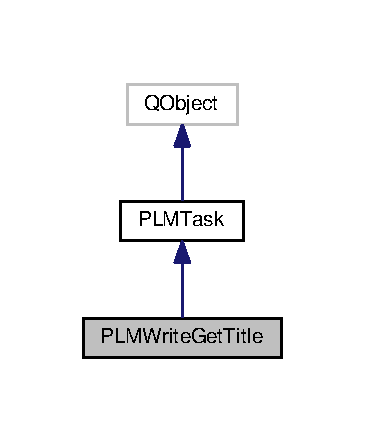
\includegraphics[width=175pt]{class_p_l_m_write_get_title__inherit__graph}
\end{center}
\end{figure}


Collaboration diagram for P\+L\+M\+Write\+Get\+Title\+:\nopagebreak
\begin{figure}[H]
\begin{center}
\leavevmode
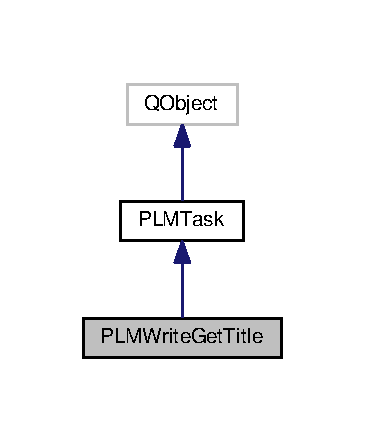
\includegraphics[width=175pt]{class_p_l_m_write_get_title__coll__graph}
\end{center}
\end{figure}
\subsection*{Public Member Functions}
\begin{DoxyCompactItemize}
\item 
{\bfseries P\+L\+M\+Write\+Get\+Title} (int project\+Id, int sheet\+\_\+id)\hypertarget{class_p_l_m_write_get_title_a8573ac331f139dc09aec755990049791}{}\label{class_p_l_m_write_get_title_a8573ac331f139dc09aec755990049791}

\item 
void {\bfseries do\+Task} (bool $\ast$ok)\hypertarget{class_p_l_m_write_get_title_a5d9f57a1b578b19735285b3d37f567bd}{}\label{class_p_l_m_write_get_title_a5d9f57a1b578b19735285b3d37f567bd}

\end{DoxyCompactItemize}
\subsection*{Additional Inherited Members}


The documentation for this class was generated from the following file\+:\begin{DoxyCompactItemize}
\item 
src/tasks/plmwritegettitle.\+h\end{DoxyCompactItemize}

\hypertarget{class_p_l_m_write_hub}{}\section{P\+L\+M\+Write\+Hub Class Reference}
\label{class_p_l_m_write_hub}\index{P\+L\+M\+Write\+Hub@{P\+L\+M\+Write\+Hub}}


Inheritance diagram for P\+L\+M\+Write\+Hub\+:\nopagebreak
\begin{figure}[H]
\begin{center}
\leavevmode
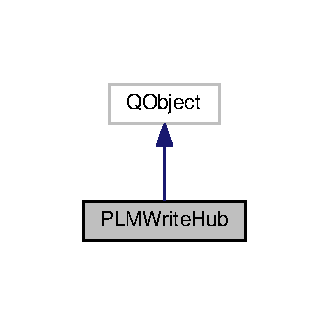
\includegraphics[width=158pt]{class_p_l_m_write_hub__inherit__graph}
\end{center}
\end{figure}


Collaboration diagram for P\+L\+M\+Write\+Hub\+:\nopagebreak
\begin{figure}[H]
\begin{center}
\leavevmode
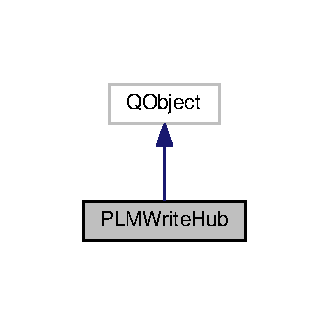
\includegraphics[width=158pt]{class_p_l_m_write_hub__coll__graph}
\end{center}
\end{figure}
\subsection*{Signals}
\begin{DoxyCompactItemize}
\item 
void {\bfseries title\+Changed} (int project\+Id, int sheet\+Id, const Q\+String \&new\+Title)\hypertarget{class_p_l_m_write_hub_a5226e205f467d69fdbbb9d16a8d01af8}{}\label{class_p_l_m_write_hub_a5226e205f467d69fdbbb9d16a8d01af8}

\end{DoxyCompactItemize}
\subsection*{Public Member Functions}
\begin{DoxyCompactItemize}
\item 
{\bfseries P\+L\+M\+Write\+Hub} (Q\+Object $\ast$parent)\hypertarget{class_p_l_m_write_hub_a554c1cae8c88cf6d645e5dec45bc9593}{}\label{class_p_l_m_write_hub_a554c1cae8c88cf6d645e5dec45bc9593}

\item 
void {\bfseries set\+Task\+Manager} (\hyperlink{class_p_l_m_task_manager}{P\+L\+M\+Task\+Manager} $\ast$task\+Manager)\hypertarget{class_p_l_m_write_hub_a8a67899963a087425b8ac703f501d665}{}\label{class_p_l_m_write_hub_a8a67899963a087425b8ac703f501d665}

\item 
Q\+List$<$ Q\+Hash$<$ Q\+String, Q\+Variant $>$ $>$ {\bfseries get\+All} (int project\+Id)\hypertarget{class_p_l_m_write_hub_a52e5b635cd12f7b6a1aba8ce2f17d64e}{}\label{class_p_l_m_write_hub_a52e5b635cd12f7b6a1aba8ce2f17d64e}

\item 
Q\+Hash$<$ int, Q\+String $>$ {\bfseries get\+All\+Titles} (int project\+Id)\hypertarget{class_p_l_m_write_hub_afde87d06c896386b118d825405ebc692}{}\label{class_p_l_m_write_hub_afde87d06c896386b118d825405ebc692}

\item 
Q\+Hash$<$ int, int $>$ {\bfseries get\+All\+Indents} (int project\+Id)\hypertarget{class_p_l_m_write_hub_a3782f562e8eded569d90c0f531f42623}{}\label{class_p_l_m_write_hub_a3782f562e8eded569d90c0f531f42623}

\item 
void {\bfseries set\+Title} (int project\+Id, int sheet\+Id, const Q\+String \&new\+Title)\hypertarget{class_p_l_m_write_hub_a0f1c5e06d781c041c599d9efd978e024}{}\label{class_p_l_m_write_hub_a0f1c5e06d781c041c599d9efd978e024}

\item 
Q\+String {\bfseries get\+Title} (int project\+Id, int sheet\+Id) const \hypertarget{class_p_l_m_write_hub_af3058a0251b7c4b667ad3db1701157aa}{}\label{class_p_l_m_write_hub_af3058a0251b7c4b667ad3db1701157aa}

\end{DoxyCompactItemize}


The documentation for this class was generated from the following files\+:\begin{DoxyCompactItemize}
\item 
src/plmwritehub.\+h\item 
src/plmwritehub.\+cpp\end{DoxyCompactItemize}

\hypertarget{class_p_l_m_write_set_title}{}\section{P\+L\+M\+Write\+Set\+Title Class Reference}
\label{class_p_l_m_write_set_title}\index{P\+L\+M\+Write\+Set\+Title@{P\+L\+M\+Write\+Set\+Title}}


Inheritance diagram for P\+L\+M\+Write\+Set\+Title\+:\nopagebreak
\begin{figure}[H]
\begin{center}
\leavevmode
\includegraphics[width=174pt]{class_p_l_m_write_set_title__inherit__graph}
\end{center}
\end{figure}


Collaboration diagram for P\+L\+M\+Write\+Set\+Title\+:\nopagebreak
\begin{figure}[H]
\begin{center}
\leavevmode
\includegraphics[width=174pt]{class_p_l_m_write_set_title__coll__graph}
\end{center}
\end{figure}
\subsection*{Public Member Functions}
\begin{DoxyCompactItemize}
\item 
{\bfseries P\+L\+M\+Write\+Set\+Title} (int project\+Id, int sheet\+\_\+id, const Q\+String \&new\+Title)\hypertarget{class_p_l_m_write_set_title_a55dc60659dfeb575438a24fa4f8f0d00}{}\label{class_p_l_m_write_set_title_a55dc60659dfeb575438a24fa4f8f0d00}

\item 
void {\bfseries do\+Task} (bool $\ast$ok)\hypertarget{class_p_l_m_write_set_title_afbd40fd05d70d914a6b005a4cbb1ee55}{}\label{class_p_l_m_write_set_title_afbd40fd05d70d914a6b005a4cbb1ee55}

\end{DoxyCompactItemize}
\subsection*{Additional Inherited Members}


The documentation for this class was generated from the following file\+:\begin{DoxyCompactItemize}
\item 
src/tasks/plmwritesettitle.\+h\end{DoxyCompactItemize}

%--- End generated contents ---

% Index
\backmatter
\newpage
\phantomsection
\clearemptydoublepage
\addcontentsline{toc}{chapter}{Index}
\printindex

\end{document}
